\documentclass[12pt]{report} % Times New Roman, 12pt

% Extra functionality for colouring elements
\usepackage[table,dvipsnames]{xcolor}

\usepackage{gscale_thesis_doublespace} % Double spaced thesis
\usepackage{fancyheadings} % Header and footer styling
\usepackage{setspace} % Allows double spacing but skips headers/footers
\setcounter{tocdepth}{1} % Limits the TOC to chapter and section names

% Additional packages
\usepackage{graphicx} % Allows the inclusion of figures
\usepackage{subcaption} % Allows captions to be added to subfigures
\usepackage[justification=centering]{caption} % Centres caption text
\usepackage{array} % Used for table formatting
\newcolumntype{P}[1]{>{\raggedright\let\newline\\\arraybackslash\hspace{0pt}}m{#1}}
\usepackage{booktabs} % Fancy-style tables
\usepackage{longtable} % Allows for tables that are more than one page long
\usepackage{float} % Better figure placement control
\usepackage{enumerate} % Numbered lists
\usepackage[shortlabels]{enumitem} % For controlling enumerate labels
\usepackage[shortcuts]{extdash} % Allows manual hyphenation of hypenated words
\usepackage{amsmath} % Non-standard math symbols
\usepackage{amsfonts} % Extended fonts for mathematics

% For nice captions and floating environments, such as for my code snippets
\usepackage{caption}
\usepackage{float}
\definecolor{darkblue}{RGB}{0,0,139}

\usepackage{todonotes}

\usepackage[newfloat=true]{minted}
\newenvironment{code}{\captionsetup{type=listing}}{}
\SetupFloatingEnvironment{listing}{name=Code, listname=List of Codes}

\usepackage{listings}
\renewcommand{\lstlistlistingname}{List of Codes}

\lstdefinelanguage{json}{
	tabsize=1,
	basicstyle=\normalfont\ttfamily,
	numbers=left,
	numberstyle=\scriptsize,
	stepnumber=1,
	numbersep=8pt,
	showstringspaces=false,
	breaklines=true,
	literate=
	{:}{{{\color{McMasterLightMaroon}{:}}}}{1}
	{,}{{{\color{McMasterLightMaroon}{,}}}}{1}
	{\{}{{{\color{McMasterWorldBlue}{\{}}}}{1}
	{\}}{{{\color{McMasterWorldBlue}{\}}}}}{1}
	{[}{{{\color{McMasterWorldBlue}{[}}}}{1}
	{]}{{{\color{McMasterWorldBlue}{]}}}}{1},
}

\lstdefinelanguage{haskell1}{
	language=haskell,
	tabsize=2,
	basicstyle=\small\ttfamily,
	numbers=left,
	numberstyle=\scriptsize,
	stringstyle=\color{orange},
	stepnumber=1,
	numbersep=8pt,
	showstringspaces=false,
	breaklines=true,
	postbreak=\mbox{\textcolor{black}{$\hookrightarrow$}\space},
	frame=lines,
	framerule=1.5pt,
	commentstyle=\color{gray},
	morecomment=[l]\--,
	keywordstyle=[1]\color{McMasterWorldGreen},
	keywords=[1]{case,class,data,deriving,do,else,if,import,qualified,in,infixl,
		infixr,instance,let,module,of,primitive,then,type,where,family,newtype,as},
	keywordstyle=[1]\color{McMasterWorldGreen},
	keywords=[2]{->,|,=>,::,[,],\,*,<-, Document, Title, Author, 
	LayoutObj, Sentence, Bool, ModelExpr, PExpr, RawContent, ListType, DType, 
	Identifier, Contents, Lbl, Filepath, MaxWidthPercent, BibRef, Maybe, Width, 
	Height, Tags, Spec, Label, Caption, Depth, String, Reference, 
	LabelledContent, PrintingInformation, D, Doc, DocSection, Intro, LearnObj, 
	Review, CaseProb, Example, Smmry, BibSec, Apndx, LsnDesc, LsnChapter, 
	LsnDecl, IdeaDict, SystemInformation, Notebook, ShowToC, Section, SecCons, 
	UnitalChunk, CI, CodeExpr, Expr, Special, LinkType, DocType, Char, Int, 
	ItemType, Ops, Variation},
	keywordstyle=[2]\color{McMasterWorldBlue},
	keywords=[3]{equationsSent, lbldExpr, unlbldExpr, lo, makeEquation, toEqn, 
	layLabelled, layUnlabelled, DocDesc, printLO, unlbldCode, rectVel},
	keywordstyle=[3]\color{McMasterHeritageMaroon},
	keywords=[4]{T, QP, P, J, NB, Lsn, CP, TeX, L, Docum},
	keywordstyle=[4]\color{blue}
 }

\usepackage[hidelinks]{hyperref} % Linking to LaTeX labels and external URLs
\hypersetup{
	colorlinks=true,
	linkcolor=black,
	urlcolor=red,
	citecolor=blue
}

\numberwithin{equation}{section} % Numbers equations based on their section

% McMaster Colours
% -- McMaster Colours --

% McMaster Palette based on https://brand.mcmaster.ca/element/colour-palette/

% Heritage Colours
\definecolor{McMasterHeritageMaroon}{HTML}{7A003C}
\definecolor{McMasterHeritageGold}{HTML}{FDBF57}
\definecolor{McMasterHeritageGrey}{HTML}{5E6A71}

% Tints and Shades
\definecolor{McMasterLightMaroon}{HTML}{ac1455}
\definecolor{McMasterDarkMaroon}{HTML}{56002a}

\definecolor{McMasterLightGrey}{HTML}{efefef}
\definecolor{McMasterCoolGrey}{HTML}{dbdbdd}
\definecolor{McMasterMediumGrey}{HTML}{aeb4b8}
\definecolor{McMasterDarkGrey}{HTML}{222222}

% Highlights
\definecolor{McMasterWorldYellow}{HTML}{FFD100}
\definecolor{McMasterWorldLime}{HTML}{D2D755}
\definecolor{McMasterWorldSkyBlue}{HTML}{8BD3E6}

% Darker Tones
\definecolor{McMasterWorldRed}{HTML}{A6192E}
\definecolor{McMasterWorldGreen}{HTML}{007B4B}
\definecolor{McMasterWorldBlue}{HTML}{007096}

\newcommand*{\macred}{\textcolor{McMasterHeritageMaroon}}
\newcommand*{\macblue}{\textcolor{McMasterWorldBlue}}

% Required for biblatex, but also adds functionality for quotation
\usepackage{csquotes}

\usepackage[
style=numeric-comp,
backend=biber,
sorting=none,
backref=true,
maxnames=99,
alldates=iso,
seconds=true
]{biblatex} % bibliography
\addbibresource{references.bib}

% ********************************
\begin{document}
\title{Generating Jupyter Notebooks in Drasil}
\halftitle{Generating Jupyter Notebooks in Drasil} % 60 Characters Max. 
%Including Spaces

\author{Ting-Yu Wu}
\shortauthor{Ting-Yu Wu} % Used for page header

\dept{Department of Computing and Software}
\field{Computing and Software} % What field your thesis is in (e.g. Software 
%Engineering)

\prevdegreeone{B.Sc. (Information \& Computer Engineering),\\Chung Yuan 
Christian University, Taoyuan, Taiwan}
\prevdegreetwo{B.Sc.} % Just your degree's field

\submitdate{April 2023} % Use the month's full spelling e.g. November
\copyrightyear{2023} % Year you are submitting this, usually your graduation 
%year

\doctype{Report} % ``Report'' or ``Thesis'' or whatever you need
\degree{Masters of Engineering} % The degree you get when you submit this
\degreeabbrv{M.Eng.}
\principaladviser{Dr. Spencer Smith and Dr. Jacques Carette} % Your Supervisor
 % LaTeX variables for preface pages/headers

\beforepreface % Half title page, title page, declaration page   
  \prefacesection{Lay Abstract}

Jupyter Notebook is a widely-used web application that enables users to create 
and share documentation, especially for scientific and engineering problems, 
due to its flexibility and ability to integrate text and code in a single 
document. To improve the efficiency of software documentation development, 
Drasil offers a framework that allows users to provide high-level information 
about their scientific problems and generates software documentation for them 
using the standardized Software Requirements Specification (SRS) template. In 
this work, we contribute to Drasil by generating Jupyter Notebooks, focusing on 
achieving three goals: generating SRS in notebook format, generating 
educational documents (i.e., lesson plans), and combining text and code in 
Drasil-generated Jupyter Notebooks. % Lay Abstract
  \prefacesection{Abstract}

Scientific Computing (SC) involves analyzing and simulating complex scientific 
and engineering problems using computing techniques and tools. To improve the 
understandability, maintainability, and reproducibility of SC software,  
documentation should be an integral part of the development process. Jupyter 
Notebook is a popular tool for developing SC software documentation, and is 
also used to enhance teaching and learning efficiency in engineering education 
due to its flexibility and benefits, such as the ability to combine text and 
code. Despite the importance of documentation, it is often missing or poorly 
executed in SC software because it is time-consuming. 

Drasil is a framework that aims to improve the efficiency of documentation 
development. By encoding each piece of information for scientific problems once 
and generating the document automatically, Drasil saves time in the 
documentation development process. We are interested in generating Jupyter 
Notebooks in Drasil to expand its applications, including generating 
educational documents.

To achieve this, we implement a JSON printer capable of generating Drasil 
software artifacts, such as Software Requirement Specifications (SRS), in 
notebook format. This enables us to generate Jupyter Notebooks in Drasil, and 
generate educational documents, starting with lesson plans. We develop the 
structure of our lesson plans and designed the language of lesson plans in 
Drasil. Additionally, Jupyter Notebooks seamlessly integrate different content 
types with code, making them ideal for data research. We explore two different 
approaches for splitting the contents. These approaches involve splitting 
content either by sections or by content types. The goal of these approaches is 
to effectively combine text and code of our Drasil-generated Jupyter Notebooks. % Abstract
  \prefacesection{Acknowledgements}

I am deeply grateful to my supervisors, Dr. Spencer Smith and Dr. Jacques 
Carette, for their support and guidance throughout this project. Their 
expertise and insights have been invaluable in shaping my research, and I could 
not have completed this work without their guidance. Their constructive 
feedback, encouragement, and patience have been truly appreciated, and I feel 
fortunate to have had the opportunity to work with them.

I would also like to express my gratitude to my colleagues, Jason Balaci, Sam 
Crawford, and Don Chen, for their willingness to share their expertise and 
knowledge. Their dedication and talent have inspired and motivated me, and I am 
grateful to have worked alongside such amazing colleagues.

Lastly, I would like to thank my parents for their unconditional love and 
unwavering support throughout my academic journey. Their encouragement have 
given me the confidence to pursue my dreams, and I am forever grateful for 
their belief in me. % Acknowledgements
  \referencepages % Table of Contents, List of Figures, List of Tables
  \lstlistoflistings
  \prefacesection{Notation and Abbreviations}

\section*{Notation}
\begin{description}[font=\rmfamily\bfseries, leftmargin=3cm, style=nextline]
	\item[$a^c$] constant acceleration
	\item[$t$] time
	\item[$v$] speed
	\item[$v^i$] initial speed
\end{description}

\section*{Abbreviations}
\begin{description}[font=\rmfamily\bfseries, leftmargin=3cm, style=nextline]
	\item[CSS] Cascading Style Sheets
	\item[GOOL] Generic Object-Oriented Language
	\item[HTML] HyperText Markup Language
	\item[IDE] Integrated Development Environment 
	\item[JSON] JavaScript Object Notation
	\item[PDF] Portable Document Format
	\item[SC] Scientific Computing
	\item[SRS] Software Requirement Specifications
\end{description}
  \academicstatement{academicachievementdeclaration}
\afterpreface  

  \chapter{Introduction} \label{chap:intro}
Scientific Computing (SC) is at the intersection of computer science, 
mathematics, and science. SC analyses and simulates mathematical methods of 
complex scientific and engineering problems by using computing techniques and 
tools. To improve understandability, maintainability, and reproducibility, 
writing documentation should be part of the process of developing scientific 
software. The role of documentation is to help people better understand the 
software and to ``communicate information to its audience and instill knowledge 
of the system it describes" \cite{forward2002software}. The significance of 
software documentation has been presented in many papers by previous 
researchers. High-quality documentation serves as the foundation for effective 
communication within software development teams, while also contributing to the 
overall excellence of the software product \cite{parnas2011precise, 
chomal2014significance, kipyegen2013importance}. Additionally, Smith et al. 
\cite{SmithandKoothoor2016, SmithandYu2007} shows that developing SC software 
in a document-driven methodology potentially improves the quality of the 
software. 

Jupyter Notebook is a popular approach for documenting SC software, providing a 
system for creating and sharing data science and scientific computing 
documentation and code. This nonprofit, open-source application was born in 
2014. Jupyter Notebook provides interactive computing across multiple 
programming languages, such as Python, Javascript, Matlab, and R. A Jupyter 
Notebook integrates text, live code, equations, computational outputs, 
visualizations, and multimedia resources, including images and videos. Jupyter 
Notebook is one of the most widely used interactive systems among scientists. 
Its popularity has grown from 200,000 to 2.5 million public Jupyter Notebooks 
on GitHub in three years from 2015 to 2018 \cite{Jeffrey2018}. It is used in a 
variety of areas and ways because of its flexibility and added values. For 
example, Notebooks can be used as an educational tool in engineering courses, 
enhancing teaching and learning efficiency \cite{cardoso2019using, zhao2019use}.

Even though the importance of documentation is widely recognized, it is often 
missing or poorly realized in SC software because: i) scientists are not aware 
of the why, how, and what of documentation \cite{hermann2022documenting, 
chang2022understanding}; ii) it is time-consuming to produce 
\cite{sanders2008dealing}; iii) scientists generally believe that writing 
documentation demands more effort and work than the benefits it would yield 
\cite{smith2016advantages}.

Jupyter Notebook simplifies the process of maintaining SC documentation by 
enabling explanatory text and code to be combined in a single document. 
Furthermore, it provides easy sharing of notebooks on platforms like GitHub and 
exportation to different formats, such as PDF. However, there are also some 
downsides to employing it. While Jupyter Notebook streamlines documenting code, 
it can be more challenging to maintain and refactor the code itself, especially 
when dealing with large datasets or complex code. Debugging and refactoring 
code across multiple segments, for instance, can be time-consuming and 
difficult to test. Poor coding practices may lead to poor quality and 
reproducibility of Jupyter Notebooks \cite{pimentel2021understanding, 
wang2020better}.

We are trying to increase the efficiency of documentation development by 
adopting generative programming. Generative programming is a technique that 
allows programmers to write the code or document at a higher abstraction level, 
and the generator produces the desired outputs. Drasil is an application of 
generative programming, and it is the framework we use to conduct this 
research. Drasil saves us more time in the documentation development process by 
letting us encode each piece of information of our scientific problems once and 
generating the document automatically.

In this chapter, we will provide an introduction to Drasil and Jupyter 
Notebook, including their usage and benefits. Following this, we will delve 
into the problems that our paper aims to address.

\section{Background}
Chapter~\ref{chap:intro_drasil} gives a general introduction to Drasil, and
Chapter~\ref{chap:intro_notebook} discusses the features and benefits of 
Jupyter Notebook.

\subsection{Drasil} \label{chap:intro_drasil}
Drasil is a framework that can generate software artifacts, including Software 
Requirement Specifications (SRS), code (C++, C\#, Java, and Python), README, 
and Makefile, from a stable knowledge base. The goals of Drasil are reducing 
knowledge duplication and improving traceability \cite{drasil}. Drasil captures 
the knowledge through our hand-made case studies. We currently have 10 case 
studies that cover different physics problems, such as Projectile motion and 
double Pendulum simulation. Recipes for scientific problems are encoded in 
Drasil, which then generates code and documentation for us. Each piece of 
information only needs to be provided to Drasil once, and that information can 
be used wherever it is needed. By defining and storing common concepts in a 
central repository and case-specific concepts in their own packages, Drasil 
enables the reuse of information across different engineering domains and 
applications. This feature significantly reduces the time and effort required 
for software development and documentation, while also improving the 
consistency and accuracy of the information being used. Later in the chapters, 
we will discuss the details of how information is encoded and how knowledge is 
reused in Drasil.

The SRS is built using a template for designing and documenting scientific 
computing software requirements as created by Smith et al \cite{smith2005new}. 
Drasil is currently capable of generating an SRS in the document languages HTML 
and LaTeX. We are looking to extend the capability of Drasil by generating 
Jupyter Notebooks in Drasil.

For more details on how to create a project using Drasil and how information is 
encoded, please refer to Chapter~\ref{chap:lessonplan} and the 
\href{https://github.com/JacquesCarette/Drasil/wiki/Creating-Your-Project-in-Drasil}{Drasil
	Wiki: Creating Your Project in Drasil}. 

\subsection{Jupyter Notebook} \label{chap:intro_notebook}
Jupyter Notebook is an interactive open-source web application for creating and 
sharing computational science documentation that contains text, executable 
code, mathematical equations, graphics, and visualizations.

\subsubsection{Structure of a notebook document}
A Jupyter Notebook has two components: front-end ``cells" and back-end 
``kernels". The notebook consists of a series of cells, which can be code 
cells, Markdown cells, or raw cells. A cell is a multiline text input field. 
The notebook follows a sequential flow, where users enter a piece of 
information, either in the form of text or programming code, into the cells 
from the web page interface. This information is then sent to the back-end 
kernels for execution, and the results are returned to the user 
\cite{notebookdoc}. Figure~\ref{fig:running_code} shows an example of a
Jupyter Notebook \cite{jupyternotebookrep}.

\begin{figure}[h!]
	\caption{Example of a Jupyter Notebook}
	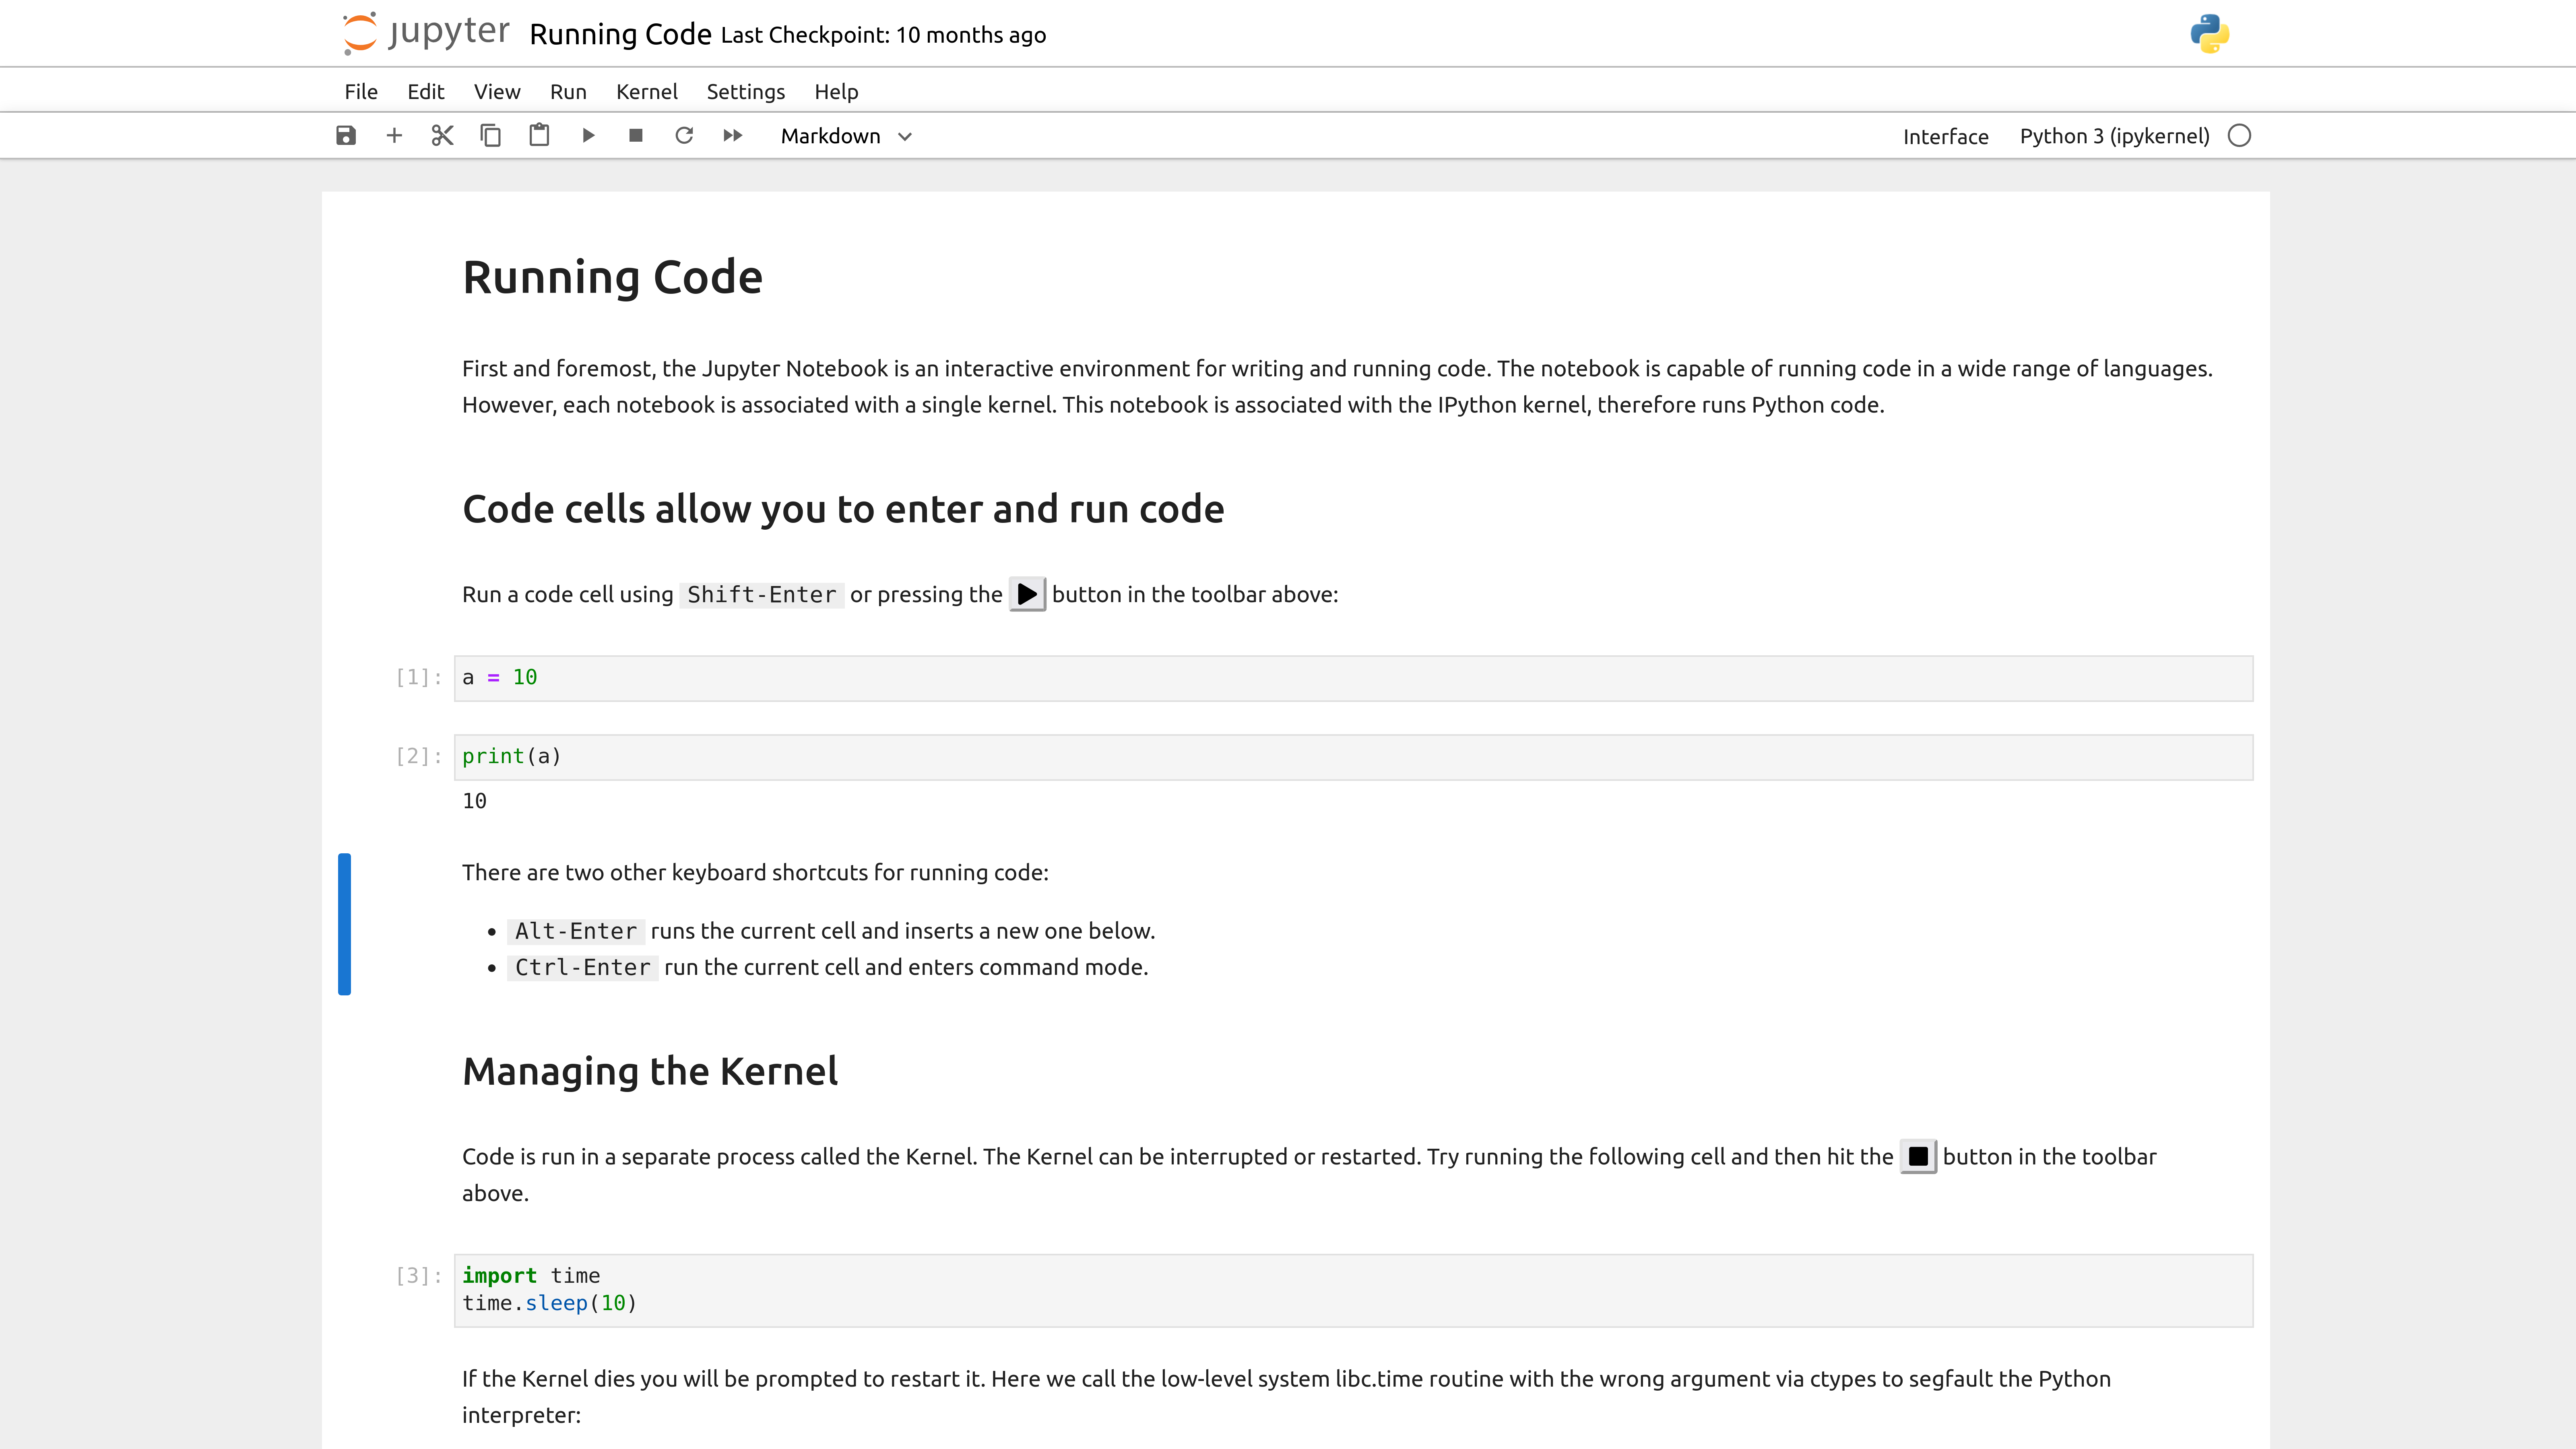
\includegraphics[width=1\textwidth]{figures/running_code.png}
	\label{fig:running_code}
\end{figure}

\subsubsection{The Value of Jupyter Notebooks}
There are several advantages of Jupyter Notebooks: sharable, all-in-one, and 
live code. First of all, the notebook is easy to share because it can be 
converted into other formats such as HTML, Markdown, and PDF. This is 
advantageuous because it allows someone working on a notebook to share it with 
others without requesting that they install any additional software and making 
it easier to collaborate on the projects. Secondly, Jupyter Notebooks combine 
all aspects of data in one single document, making the document easy to 
visualize, maintain and modify. In addition, they provide an environment of 
live code and computational equations. Usually, when programmers are running 
code on some other IDEs, they have to write the entire program before executing 
it. However, the notebook allows programmers to execute a specific portion of 
the code without running the whole program. The ability to run a snippet of 
code and integrate with text highlight the usability of the notebook. Previous 
research has demonstrated that Jupyter Notebooks can significantly contribute 
to reproducibility, reusability, and more effective computational workflows in 
science \cite{beg2021using}.

\section{Problem Statement}
Since both Jupyter Notebook and Drasil focus on creating and generating 
scientific computing documentation, we are interested in extending the values 
of Jupyter Notebook to Drasil and the kind of knowledge we can manipulate. 
Following are the three main problems we are trying to solve with Drasil in 
this paper:

\begin{enumerate}
	\item Generate Jupyter Notebooks. To acheive this, we will have 
	to generate documents in notebook format. Jupyter Notebook is a simple 
	JSON document with a .ipynb file extension. Notebook contents are either 
	code or Markdown. Therefore, non-code contents must be in Markdown format 
	with JSON layout. Drasil can currently write in HTML and LaTeX. We are 
	building a notebook printer in Drasil for generating documents that are 
	readable and writable in Jupyter Notebook.
	\item Develop the structure of lesson plans and generate them. As 
	mentioned, Jupyter Notebook is used as an educational tool for teaching 
	engineering courses. When it comes to teaching, lesson plans are often 
	brought up because they help teachers to organize the daily activities 
	in each class time. We are interested in teaching Drasil a ``textbook" 
	structure by starting with generating a simple physics lesson plan and 
	expanding Drasil's application. We aim to capture the elements of 
	textbook chapters, identify the family of lesson plans, and classify the 
	knowledge to build a general structure in Drasil, which will enable the 
	lesson plan to generalize to a variety of lessons.
	\item Generate notebooks that mix text and Python code. Jupyter Notebook is 
	an interactive application for creating documents that contain formattable 
	text and executable code. However, Drasil doesn't currently support 
	interactive recipes. There is no code in SRS documents, and text and code 
	are generated separately in Drasil. We are looking for the possibility of 
	generating a notebook document that incorporate both text and Python code, 
	thereby	enhancing the capabilities of Drasil and its potential to solve 
	more scientific problems.
\end{enumerate}

\section{Thesis Outline}
Chapter~\ref{chap:nbprinter} covers the topic of how Drasil generates and 
prints documents using the Drasil printer, as well as the creation of the 
notebook printer for generating Jupyter Notebooks in Drasil. Moving on to 
Chapter~\ref{chap:lessonplan}, we discuss the structure of lesson plans, how we 
define the lesson plans language in Drasil, and how to generate them with the 
notebook printer. Chapter~\ref{chap:codeBlock} discusses various approaches for 
splitting the contents to mix different types of content, such as text and 
code, in Jupyter Notebooks with Drasil, as well as the implementation for 
generating code blocks. Lastly, Chapter~\ref{chap:conclusion} provides an 
overview of the future work and concludes the achievements of this work.
\chapter{Drasil Printer} \label{chap:nbprinter}
To generate Jupyter Notebooks in Drasil, the first step is to build a printer 
that can handle notebook generation. As explained in Chapter~\ref{chap:intro}, 
a notebook is a JSON document composed of code and Markdown contexts, such as 
text and images. Drasil is currently capable of generating SRS documents in 
HTML and LaTeX, which are handled by the HTML and TeX printers, respectively. 
We are adding a JSON printer to Drasil for generating SRS documents in notebook 
format.

Once we have the user-encoded document (i.e., recipes of the scientific 
problem), the contents are passed to Drasil's printers for printing. 
The printer is located in the \textbf{drasil-printers}, which contains all the 
necessary modules and functions for printing software artifacts. The 
\textbf{drasil-printers} module is responsible for transferring the types and 
data defined in Drasil's source language to printable objects and rendering 
those objects in desirable formats, such as HTML, LaTeX, or JSON. A list of 
packages and modules of the printers and their responsibilities can be found in 
Table~\ref{tab:printerpacks}. The majority of the \textbf{drasil-printers} 
already existed before this research; we only added a JSON printer and made a 
few changes to it for better notebook printing.

This chapter explains how the contents are printed, how the printer works, and 
the implementation of the JSON printer.

\begin{longtable}[c]{|>{\raggedright}p{0.32\linewidth}|>{\raggedright\arraybackslash}p{0.61\linewidth}|}
	\caption{Summary of Packages and Modules in drasil-printers} 
	\label{tab:printerpacks}                                              
	\\ \hline
	
	\rowcolor{McMasterMediumGrey}
	\textbf{Package/Module} & \textbf{Responsibility}
	\\ \hline
	
	Language.Drasil.DOT & Defines types and holds functions for generating 
	traceability graphs as .dot files. 
	\\ \hline
	Language.Drasil.HTML & Holds all functions needed to generate HTML files. 
	\\ \hline
	Language.Drasil.JSON & Holds all functions needed to generate JSON files. 
	\\ \hline
	Language.Drasil.Log & Holds functions for generating log files. 
	\\ \hline
	Language.Drasil.Markdown & Holds functions for generating READMEs alongside 
	GOOL code.
	\\ \hline
	Language.Drasil.Plain & Holds functions for generating plain files.
	\\ \hline
	Language.Drasil.Printing & Transfers types and datas to printable objects 
	and defines helper functions for printing.
	\\ \hline
	Language.Drasil.TeX & Holds all functions needed to generate TeX files. 
	\\ \hline
	Language.Drasil.Config & Holds default configuration functions. 
	\\ \hline
	Language.Drasil.Format & Defines document types (SRS, Website, or Jupyter) 
	and output formats (HTML, TeX, JSON, or Plain).
	\\ \hline
\end{longtable}

\section{How documents are printed in Drasil}
In Drasil, a document that is meant to be printable includes a title, authors, 
and layout objects, as illustrated in Code~\ref{code:Document}. While the title 
and authors are simply of type \texttt{Sentence}, the layout objects are a 
collection of various contents.

\begin{listing}[h]
	\caption{Source Code for Definition of a Printable Document}
	\label{code:Document}
	\begin{lstlisting}[language=haskell1]
		data Document = Document Title Author [LayoutObj]
	\end{lstlisting}
\end{listing}

The contents of the document are defined as \texttt{RawContent} in Drasil's 
document source language, as shown in Code~\ref{code:RawContent}. We categorize 
the contents into various types and deal with them explicitly. For instance, a 
\texttt{Paragraph} is comprised of sentences, and an \texttt{EqnBlock} holds an 
expression of type \texttt{ModelExpr}\footnote{\texttt{ModelExpr} is a 
mathematical expression language.}. 

\begin{listing}[h]
	\caption{Source Code for Definition of RawContent}
	\label{code:RawContent}
	\begin{lstlisting}[language=haskell1]
		-- | Types of contents we deal with explicitly.
		data RawContent =
		Table [Sentence] [[Sentence]] Title Bool
		| Paragraph Sentence                       
		| EqnBlock ModelExpr                      
		| DerivBlock Sentence [RawContent]        
		| Enumeration ListType                    
		| Defini DType [(Identifier, [Contents])] 
		| Figure Lbl Filepath MaxWidthPercent     
		| Bib BibRef                              
		| Graph [(Sentence, Sentence)] (Maybe Width) (Maybe Height) Lbl
	\end{lstlisting}
\end{listing}

To print these raw contents, we transform them into printable layout objects, 
defined in Code~\ref{code:LayoutObj} in \textbf{Language.Drasil.Printing}. 
Although the types of these layout objects are similar to the types of the raw 
contents, layout objects are more appropriate for printing because all the 
information is generalized into a type called \texttt{Spec}, as shown in 
Code~\ref{code:Spec}. For example, a printable \texttt{Paragraph} contains 
\texttt{Contents}, which is a \texttt{Spec} (Code~\ref{code:Contents}). The 
smallest unit that any layout object holds is always a \texttt{Spec}, which 
means that printing always starts from a \texttt{Spec}. By generalizing  
different kinds of information that layout objects hold, we can print them more 
efficiently. 

\begin{listing}[h]
	\caption{Source Code for Definition of LayoutObj}
	\label{code:LayoutObj}
	\begin{lstlisting}[language=haskell1]
		-- | Defines types similar to content types of 
		-- RawContent in "Language.Drasil" but better 
		-- suited for printing.
		data LayoutObj = 
				Table Tags [[Spec]] Label Bool Caption                          
			| Header Depth Title Label                                       
			| Paragraph Contents                                              
			| EqnBlock Contents                                               
			| Definition DType [(String,[LayoutObj])] Label                   
			| List ListType                                                   
			| Figure Label Caption Filepath MaxWidthPercent                  
			| Graph [(Spec, Spec)] (Maybe Width) (Maybe Height) Caption Label 
			| HDiv Tags [LayoutObj] Label                                    
			| Cell [LayoutObj] 
			| Bib BibRef         
	\end{lstlisting}
\end{listing}

\begin{listing}[h!]
	\caption{Source Code for Definition of Spec}
	\label{code:Spec}
	\begin{lstlisting}[language=haskell1]
		-- | Redefine the 'Sentence' type from Language.Drasil 
		-- to be more suitable to printing.
		data Spec = E Expr                   
							| S String                
							| Spec :+: Spec          
							| Sp Special              
							| Ref LinkType String Spec 
							| EmptyS                  
							| Quote Spec              
							| HARDNL                 
	\end{lstlisting}
\end{listing}

\begin{listing}[h!]
	\caption{Source Code for Definition of Contents}
	\label{code:Contents}
	\begin{lstlisting}[language=haskell1]
		-- | Contents are just a sentence ('Spec').
		type Contents = Spec       
	\end{lstlisting}
\end{listing}

Once the conversion of contents from \texttt{RawContent} to 
\texttt{LayoutObj} is done, the layout objects can be targeted to 
produce the desired format in various document languages through language 
printers.

Here is an example of how an expression is encoded and printed: 
Equation~\ref{eq:velocity} represents the velocity ($v$) obtained by 
integrating constant acceleration ($a^c$) with respect to time ($t$) in one 
dimension, which is used in the case study 
\href{https://jacquescarette.github.io/Drasil/examples/projectile/SRS/srs/Projectile_SRS.html}{Projectile}:
 
\begin{equation}
	\label{eq:velocity}
	v=v^i+a^ct
\end{equation}

To encode Equation~\ref{eq:velocity}, which we name \texttt{rectVel}, we 
might write it as shown in Code~\ref{code:encodeProjExpr}, where the type 
\texttt{pExpr} is a synonyms used for \texttt{ModelExpr}. Let's unpack this 
code. The \texttt{QP} module is located in 
\textbf{Data.Drasil.Quantities.Physics} and is responsible for assigning 
symbols and units to physical concepts used in Drasil, including time, speed, 
acceleration, and gravity. These quantities are of type 
\texttt{UnitalChunk}\footnote{\texttt{UnitalChunk}s are concepts with 
quantities that require a definition of units. A \texttt{UnitalChunk} contains 
a `Concept', `Symbol', and `Unit'.}, which represents concepts with quantities 
that require a unit definition. For example, \texttt{constAccel} is a physical 
concept with the definition ``a one-dimensional acceleration that is 
constant'', symbol $a^c$, and unit $m/s$.
 
The \texttt{sy} constructor creates an expression from a concept that contains 
a symbol. Additionally, it is clear that \texttt{\$=}, \texttt{addRe}, and 
\texttt{mulRe} constructors are used for equating, adding, and multiplying two 
expressions, respectively.

\begin{listing}[h]
	\caption{Code for Encoding rectVel}
	\label{code:encodeProjExpr}
	\begin{lstlisting}[language=haskell1]
		rectVel :: PExpr
		rectVel = sy QP.speed $= sy QP.iSpeed `addRe` 
		(sy QP.constAccel `mulRe` sy QP.time)
	\end{lstlisting}
\end{listing}

Once the equation is defined, we can incorporate it into a \texttt{Sentence}. 
Code~\ref{code:ExprtoSent} shows an example of using an expression in a 
sentence, where \texttt{eS} lifts a \texttt{ModelExpr} to a 
\texttt{Sentence}. Equations can also be used in other content types that 
contain expressions, such as \texttt{DerivBlock}\footnote{\texttt{DerivBlock} 
is a type of contents representing a derivation block.}. Alternatively, we can 
convert expressions directly to \texttt{Contents}, as shown in 
Code~\ref{code:ExprtoCont}.

\begin{listing}[h]
	\caption{Code for Converting rectVel to a Sentence}
	\label{code:ExprtoSent}
	\begin{lstlisting}[language=haskell1]
		equationsSent :: Sentence
		equationsSent = S "From Equation" +:+ eS rectVel
	\end{lstlisting}
\end{listing}

\begin{listing}[h]
	\caption{Source Code for Converting ModelExpr to Contents}
	\label{code:ExprtoCont}
	\begin{lstlisting}[language=haskell1]
		-- | Displays a given expression and attaches a 'Reference' to it.
		lbldExpr :: ModelExpr -> Reference -> LabelledContent
		lbldExpr c lbl = llcc lbl $ EqnBlock c
		
		-- | Same as 'lbldExpr' except content is unlabelled 
		-- (does not attach a 'Reference').
		unlbldExpr :: ModelExpr -> Contents
		unlbldExpr c = UlC $ ulcc $ EqnBlock c
	\end{lstlisting}
\end{listing}

After encoding the equation and creating the sentence, the printers take over 
and convert the expression to a printable \texttt{EqnBlock}, which can then be 
generated in a specific document language. In Code~\ref{code:EqnblocktoTex]}, 
we can see how an \texttt{EqnBlock} is converted from a \texttt{RawContent} to 
a printable \texttt{LayoutObj} and rendered in LaTeX.

\begin{listing}
	\caption{Source Code for Rendering EqnBlock to LaTeX}
	\label{code:EqnblocktoTex]}
	\begin{lstlisting}[language=haskell1]
		-- Line 2-15 is handled by Language.Drasil.Printing
		-- | Helper that translates 'LabelledContent's to a 
		-- printable representation of 'T.LayoutObj'. 
		-- Called internally by 'lay'.
		layLabelled :: PrintingInformation -> LabelledContent -> T.LayoutObj
		layLabelled sm x@(LblC _ (EqnBlock c)) = 
			T.HDiv ["equation"] [T.EqnBlock 
			(P.E (modelExpr c sm))] (P.S $ getAdd $ getRefAdd x)
		
		-- | Helper that translates 'RawContent's to a  
		-- printable representation of 'T.LayoutObj'. 
		-- Called internally by 'lay'.
		layUnlabelled :: PrintingInformation -> RawContent -> T.LayoutObj
		layUnlabelled sm (EqnBlock c) = T.HDiv ["equation"] 
		 [T.EqnBlock	(P.E (modelExpr c sm))] P.EmptyS
		
		-- Line 18-28 is handled by Language.Drasil.TeX
		-- | Helper for rendering 'LayoutObj's into TeX.
		lo :: LayoutObj -> PrintingInformation -> D
		lo (EqnBlock contents) _ = makeEquation contents
		
		-- | Prints an equation.
		makeEquation :: Spec -> D
		makeEquation contents = toEqn (spec contents)
		
		-- | toEqn inserts an equation environment.
		toEqn :: D -> D
		toEqn (PL g) = equation $ PL (\_ -> g Math)
	\end{lstlisting}
\end{listing}

\section{Notebook Printer}
Since \texttt{LayoutObj} is the key to handling different types of contents, 
each document language's printer is responsible for rendering layout objects in 
that particular language and generating necessary information for the document. 
For example, CSS describes the style and presentation of an HTML page, so 
generating the necessary CSS selectors in HTML documents is handled by the HTML 
printer. In the case of a Jupyter Notebook document, 
metadata\footnote{Information about a book or its contents is known as 
metadata. It's often used to regulate how the notebook behaves and how its 
feature works \cite{notebookmetadata}.} is required. To implement a 
well-functioning notebook printer, our focus is on rendering contents in JSON 
format and generating necessary metadata.

\begin{listing}[h]
	\caption{Source Code for Rendering LayoutObjs into JSON}
	\label{code:LOtoJSON}
	\begin{lstlisting}[language=haskell1]
		-- | Helper for rendering LayoutObjects into JSON
		printLO :: LayoutObj -> Doc
		printLO (Header n contents l) = nbformat empty $$ nbformat 
		(h (n + 1) <> pSpec contents) $$ refID (pSpec l)
		printLO (Cell layObs) = markdownCell $ vcat (map printLO layObs)
		printLO (HDiv _ layObs _) = vcat (map printLO layObs) 
		printLO (Paragraph contents) = nbformat empty $$
		nbformat (stripnewLine (show(pSpec contents)))
		printLO (EqnBlock contents)  = nbformat mathEqn
		where
		toMathHelper (PL g) = PL (\_ -> g Math)
		mjDelimDisp d = text "$$" <> stripnewLine (show d) <> text "$$" 
		mathEqn = mjDelimDisp $ printMath $ toMathHelper $ 
		TeX.spec contents
		printLO (Table _ rows r _ _) = nbformat empty $$
		makeTable rows (pSpec r)
		printLO (Definition dt ssPs l) = nbformat (text "<br>") $$ 
		makeDefn dt ssPs (pSpec l)
		printLO (List t) = nbformat empty $$ makeList t False
		printLO (Figure r c f wp) = makeFigure (pSpec r) (pSpec c) (text f) wp
		printLO (Bib bib) = makeBib bib
		printLO Graph{} = empty 
	\end{lstlisting}
\end{listing}

\subsection{Rendering LayoutObjs in Notebook Format}
Code~\ref{code:LOtoJSON} shows the primary function for rendering layout 
objects into a notebook. This function works similarly to the ones used by the 
HTML and TeX printers, and is responsible for generating content in the 
appropriate format. Each type of layout object is handled explicitly, taking 
into account how notebook users add content by hand in Jupyter Notebook, to 
ensure accurate reproduction and display of the contents. To help us properly 
render content in notebook format, we also created a few helper functions. For 
instance, \texttt{nbformat} (Code~\ref{code:nbformat}) helps create the 
necessary indentations for each line of content and encode them into JSON. We 
take advantage of the \textbf{encode} function from the Haskell package 
\textbf{Text.JSON}, which takes a Haskell value and converts it into a JSON 
string \cite{textdotjosn}. 

\begin{listing}[h]
	\caption{Source Code for Converting Contents into JSON}
	\label{code:nbformat}
	\begin{lstlisting}[language=haskell1]
		import qualified Text.JSON as J (encode) 
		
		-- | Helper for converting a Doc in JSON format
		nbformat :: Doc -> Doc
		nbformat s = text ("    " ++ J.encode (show s ++ "\n") ++ ",")
	\end{lstlisting}
\end{listing}

In addition, because non-code contents in Jupyter Notebook are built in 
Markdown, some types of contents require special treatment for Markdown 
generation, such as tables. Although Jupyter Notebook supports HTML tables 
(where we would be able to reuse the function from the HTML printer), we want 
to make the generated documents more ``human-like" and reflect how people 
create contents in Jupyter. Therefore, instead of generating HTML tables, we 
create tables in Markdown format. The function \texttt{makeTable} from 
Code~\ref{code:makeTable} generates a table in Markdown and converts it to the
notebook format.

\begin{listing}[h!]
	\caption{Source Code for Rendering a Markdown Table}
	\label{code:makeTable}
	\begin{lstlisting}[language=haskell1]
		-- | Renders Markdown table, called by 'printLO'
		makeTable :: [[Spec]] -> Doc -> Doc
		makeTable [] _      = error "No table to print"
		makeTable (l:lls) r = refID r $$ nbformat empty $$ 
			(makeHeaderCols l $$ makeRows lls) $$ nbformat empty
		
		-- | Helper for creating table rows
		makeRows :: [[Spec]] -> Doc
		makeRows = foldr (($$) . makeColumns) empty
		
		-- | makeHeaderCols: Helper for creating table header
		-- (each of the column header cells)
		-- | makeColumns: Helper for creating table columns
		makeHeaderCols, makeColumns :: [Spec] -> Doc
		makeHeaderCols l = nbformat (text header) $$ 
			nbformat (text $ genMDtable ++ "|")
			where 
				header = show(text "|" <> hcat(punctuate 
					(text "|") (map pSpec l)) <> text "|")        
				c = count '|' header
				genMDtable = concat (replicate (c-1) "|:--- ")
		
		makeColumns ls = nbformat (text "|" <> hcat(punctuate 
			(text "|") (map pSpec ls)) <> text "|")
	\end{lstlisting}
\end{listing}

To handle the various types of contents, we break them down into different 
types and handle each type individually in our code. When we encounter a more 
complex case, we create a specific \textbf{make} function to deal with it to 
reduce confusion in the main \texttt{printLO} function. For instance, 
we have \texttt{makeTable}, which handles table generation, and 
\texttt{makeList}, which generates a list of items. These functions are then 
called by \texttt{printLO}. We carefully consider how contents are created in 
the notebook and render each type of layout object in notebook format to ensure 
that the generated document is a valid Jupyter Notebook.

\subsection{Metadata Generation}
There are two types of metadata in a Jupyter Notebook: the first type is for 
the notebook environment setup (line 9-30 in Code~\ref{code:notebookmetada} in 
Appendix A), while the second type (line 3-7 in Code~\ref{code:notebookmetada} 
in Appendix A) is used to control the behavior of a notebook cell, where we 
define the type of cell (i.e, Code or Markdown). Generating the first type of 
metadata is straightforward since the metadata for setting up the environment 
is identical across all notebooks. We built a helper function called 
\texttt{makeMetadata} to generate the necessary metadata of a notebook 
document, as shown in Code~\ref{code:makeMetadata}. This function is called 
when a notebook document is being built, and the metadata is printed at the end 
of the document. It is important to note that this metadata enables Python 
code for the generated notebook, but Jupyter Notebook also supports other 
programming languages like Matlab and R. Therefore, we plan to make other 
languages available in the future.

\begin{listing}[h!]
	\caption{Source Code for Making Metadata}
	\label{code:makeMetadata}
	\begin{lstlisting}[language=haskell1]
		-- | Generate the necessary metadata for a notebook document.
		makeMetadata :: Doc  
		makeMetadata = vcat [
			text " \"metadata\": {", 
			vcat[
				text "  \"kernelspec\": {", 
				text "   \"display_name\": \"Python 3\",", 
				text "   \"language\": \"python\",",
				text "   \"name\": \"python3\"", 
				text "  },"],
			vcat[
				text "  \"language_info\": {", 
				text "   \"codemirror_mode\": {", 
				text "    \"name\": \"ipython\",",
				text "    \"version\": 3",
				text "   },"],
			text "   \"file_extension\": \".py\",", 
			text "   \"mimetype\": \"text/x-python\",",					
			text "   \"name\": \"python\",",
			text "   \"nbconvert_exporter\": \"python\",",
			text "   \"pygments_lexer\": \"ipython3\",",
			text "   \"version\": \"3.9.1\"",
			text "  }",
			text " },",
			text " \"nbformat\": 4,", 
			text " \"nbformat_minor\": 4" 
		]
	\end{lstlisting}
\end{listing}

The second type of metadata is more complex. We need to break down our contents 
into units and differentiate them to generate the right type of cells. We will 
discuss this further in Chapter~\ref{chap:codeBlock} after introducing a new 
case study in Chapter~\ref{chap:lessonplan}. For now, since there is no code in 
the SRS, all contents should be in Markdown. To generate the metadata for a 
Markdown cell, we use the helper function \texttt{markdownCell} function from 
Code~\ref{code:markdownCell}. This function creates the necessary metadata and 
a cell for the given unit of content. An example implementation can be found in 
Code~\ref{code:callmarkdownCell}.

\begin{listing}[h]
	\caption{Source Code for markdownCell}
	\label{code:markdownCell}
	\begin{lstlisting}[language=haskell1]
		-- | Helper for building markdown cells
		markdownB', markdownE :: Doc
		markdownB' = text "  {\n   \"cell_type\": \"markdown
			\",\n \"metadata\": {},\n   \"source\": [" 
		markdownE  = text "    \"\\n\"\n   ]\n  },"
			
		-- | Helper for generate a Markdown cell
		markdownCell :: Doc -> Doc
		markdownCell c = markdownB' <> c <> markdownE
	\end{lstlisting}
\end{listing}

\begin{listing}[h]
	\caption{Source Code for Calling markdownCell}
	\label{code:callmarkdownCell}
	\begin{lstlisting}[language=haskell1]
		printLO (Cell layoutObs) = markdownCell $ vcat (map printLO layoutObs)
	\end{lstlisting}
\end{listing}

The JSON printer implemented so far is not without flaws, there is always room 
for improvement. Nevertheless, the current implementation already enables 
Drasil to generate Jupyter Notebooks and expand the generated document to 
include SRS in JSON format. This makes it possible to edit and share 
Drasil-generated documents with Jupyter Notebook, thereby increasing their 
value.
 
For complete implementation of the JSON printer, please refer to 
Code~\ref{code:JSONPrint} and Code~\ref{code:JSONHelpers} in Appendix A .
\chapter{Lesson Plans} \label{chap:lessonplan}
With the addition of a JSON printer capable of generating Jupyter Notebooks, we 
are now looking to expand Drasil's application by generating educational 
documents. As discussed in Chapter~\ref{chap:intro}, Jupyter Notebooks are 
commonly used in teaching engineering courses due to their characteristics and 
advantages. One of the educational practices to enhance teaching is creating 
lesson plans \cite{cicek2013effective, wong2018first}, which provide a 
guide for structuring daily activities in each class period. A lesson plan 
outlines the learning objectives, methods and procedures for achieving them, 
and metrics for student progress. Lesson plans are an ideal starting 
point for generating educational documents in Drasil because they are more 
accessible than academic papers. In addition, we are able to work with real 
examples in a lesson plan. 

To incorporate lesson plans in Drasil, we first need to understand their 
components and categorize the knowledge in a structured manner. We analyzed the 
similarities and differences of elements in textbook chapters in 
\href{https://github.com/smiths/caseStudies/blob/master/CaseStudies/projectile/projectileLesson/AboutProjectileLesson.pdf}{Discussion
 of Projectile Lesson: What and	Why} using online resources. Based on our 
analysis, we narrowed down the elements and defined a structure that fits our 
lesson plans the most, as summarized in Table~\ref{tab:lessonPlanstrucutre}. 
While not all chapters are mandatory, a typical lesson plan includes learning 
outcomes (objectives), lesson topics (case problems), and activities (examples).
It's worth noting that this structure may be subject to future modifications to 
better suit our needs. 

\begin{longtable}[c]{|>{\raggedright}p{0.25\linewidth}|>{\raggedright\arraybackslash}p{0.7\linewidth}|}
	\caption{Structure of Lesson Plans} 
	\label{tab:lessonPlanstrucutre}                                            
	\\ \hline
	
	\rowcolor{McMasterMediumGrey}
	\textbf{Chapter} & \textbf{Overview}
	\\ \hline
	
	Introduction & An introduction of the lesson plan or the topic.
	\\ \hline
	Learning Objectives & What students can do or will learn after the 
	lesson.  
	\\ \hline
	Review & A recap of what has been covered previously.
	\\ \hline
	A Case Problem & A case problem that link the topic to a real world 
	problem.
	\\ \hline
	Example & An example of the case problem.
	\\ \hline
	Summary & A summary of the lesson plan.
	\\ \hline
	Bibliography & References that support the lesson plan.
	\\ \hline
	Appendix & Additional resources or information of the lesson.
	\\ \hline
\end{longtable}

In this chapter, we will discuss the language of lesson plans in Drasil, 
introduce a new case study on Projectile Motion Lesson, and explore the reuse 
of knowledge in Drasil.

\section{Language of Lesson Plans} \label{chap:lessonLang}
To generate a new type of document, lesson plans, in Drasil, we must define its 
language first. Drasil's document language has SRS, and we are creating a 
language for lesson plans. As discussed in Chapter~\ref{chap:nbprinter}, a 
Drasil document has a title, authors, and sections, which hold the contents 
of the document. The definition of a document is defined in 
\textbf{drasil-lang}\footnote{\textbf{drasil-lang} holds the higher level 
language for Drasil.} as shown in 
Code~\ref{code:drasil-lang-document}\footnote{\texttt{ShowToC} is 
\texttt{ShowTableOfContents} in the source code, which is to determine whether 
to show the table of contents in the document.}, where \texttt{Document} is the 
type for SRS document and \texttt{Notebook} is for Jupyter Notebook, 
specifically lesson plans at this moment. The reason why we define them 
separately is because we print the SRS and lesson plans differently. We are 
able to pattern match the way we print the document in the printer.

\begin{listing}[h]
	\caption{Code for Definition of Document}
	\label{code:drasil-lang-document}
	\begin{lstlisting}[language=haskell1]
		data Document = Document Title Author ShowToC [Section]
									| Notebook Title Author [Section]
	\end{lstlisting}
\end{listing}

We need to create helper types and functions that facilitate the creation of 
document language for generating lesson plans, based on our lesson plans 
structure. Our first step is to define the types and data for the lesson and 
its chapters in Drasil's document language, \textbf{drasil-docLang}. 
Code~\ref{code:core} is the core declaration of the lesson plan. A 
\texttt{LsnDesc} type represents a lesson description (line 1), which consists 
of lesson chapters (line 3), including an introduction, learning objectives, 
review, case problem, example, summary, bibliography, and appendix. The detail 
structure of each chapter is defined in line 12-31. At present, 
\texttt{Contents} is the only defined elements as the chapter structure has not 
yet been fully understood. We intend to further develop the chapter structure 
in the future.

\begin{listing}[h!]
	\caption{Source Code for Notebook Core Language}
	\label{code:core}
	\begin{lstlisting}[language=haskell1]		
		type LsnDesc = [LsnChapter]

		data LsnChapter = Intro Intro
										| LearnObj LearnObj
										| Review Review
										| CaseProb CaseProb
										| Example Example
										| Smmry Smmry
										| BibSec
										| Apndx Apndx
		
		-- ** Introduction
		newtype Intro = IntrodProg [Contents]		
		-- ** Learning Objectives
		newtype LearnObj = LrnObjProg [Contents]		
		-- ** Review Chapter
		newtype Review = ReviewProg [Contents]		
		-- ** A Case Problem
		newtype CaseProb = CaseProbProg [Contents]		
		-- ** Examples of the lesson
		newtype Example = ExampleProg [Contents]		
		-- ** Summary
		newtype Smmry = SmmryProg [Contents]		
		-- ** Appendix
		newtype Apndx = ApndxProg [Contents]
	\end{lstlisting}
\end{listing}

The \texttt{LsnDecl} type, as shown in Code~\ref{code:LsnDecl}, is used to 
declare all the necessary chapters for a lesson plan. It is similar in 
definition to \texttt{LsnDesc}, but in a more usable form. It is meant to be a 
semantic rendition of a lesson plan document, while \texttt{LsnDesc} is 
intended to be a general description and more suitable for printing 
\cite{lsnDeclandlsnDesc}. They are identical at this point because the chapter 
structure is not well understood, but they might evolve differently as we gain 
more understanding of our lesson plans.

\begin{listing}[h]
	\caption{Source Code for LsnDecl}
	\label{code:LsnDecl}
	\begin{lstlisting}[language=haskell1]
		type LsnDecl  = [LsnChapter]
		
		data LsnChapter = Intro NB.Intro
										| LearnObj NB.LearnObj
										| Review NB.Review
										| CaseProb NB.CaseProb
										| Example NB.Example
										| Smmry NB.Smmry
										| BibSec
										| Apndx NB.Apndx
	\end{lstlisting}
\end{listing}

\begin{listing}[h!]
	\caption{Source Code for Section and the section Constructor}
	\label{code:section}
	\begin{lstlisting}[language=haskell1]
		data Section = Section
								  { tle  :: Title
								  , cons :: [SecCons]
								  , _lab :: Reference
								  }
		makeLenses ''Section
		
		-- | Constructor for creating 'Section's with a title 
		-- ('Sentence'), introductory contents, a list of 
		-- subsections, and a	shortname ('Reference').
		section :: Sentence -> [Contents] -> [Section] -> Reference -> Section
		section title intro secs = Section title (map Con intro ++ map Sub secs)
	\end{lstlisting}
\end{listing}

Next, we need functions to generate chapters. We can use the \texttt{Section} 
type that is used for creating SRS sections, which consists of a title, a list 
of contents, and a short name, as shown in Code~\ref{code:section}. We can also 
take advantage of the \texttt{section} smart constructor to build our own 
chapter constructors, as illustrates in Code~\ref{code:chapterConstructor}. 
Once we have these constructors, we can use them to build each chapter 
(Code~\ref{code:mkChapters}).

\begin{listing}[h!]
	\caption{Source Code for Chapter Constructors} 
	\label{code:chapterConstructor}
	\begin{lstlisting}[language=haskell1]
		learnObj, review, caseProb, example :: [Contents] -> 
				[Section] -> Section
		learnObj cs ss = section (titleize' Docum.learnObj) cs ss learnObjLabel
		review   cs ss = section (titleize Docum.review)    cs ss reviewLabel
		caseProb cs ss = section (titleize Docum.caseProb)  cs ss caseProbLabel
		example  cs ss = section (titleize Docum.example)   cs ss exampleLabel
	\end{lstlisting}
\end{listing}

\begin{listing}[h!]
	\caption{Source Code for Making Chapters} 
	\label{code:mkChapters}
	\begin{lstlisting}[language=haskell1]				
		-- | Helper for making the 'Learning Objectives'.
		mkLearnObj :: LearnObj -> Section
		mkLearnObj (LrnObjProg cs) = Lsn.learnObj cs []
		
		-- | Helper for making the 'Review'.
		mkReview :: Review -> Section
		mkReview (ReviewProg r) = Lsn.review r [] 
		
		-- | Helper for making the 'Case Problem'.
		mkCaseProb :: CaseProb -> Section
		mkCaseProb (CaseProbProg cp) = Lsn.caseProb cp [] 
		
		-- | Helper for making the 'Example'.
		mkExample:: Example -> Section
		mkExample (ExampleProg cs) = Lsn.example cs []
	\end{lstlisting}
\end{listing}

When building lesson plans, the document and chapters are encoded in the 
\texttt{LsnDecl} type, which is then converted to \texttt{LsnDesc} for 
printing. The \texttt{mkNb} function, as shown in Code~\ref{code:mkNb}, takes 
the user-encoded list of chapters (i.e., \texttt{LsnDecl}) and \texttt{System 
Information}\footnote{System Information is a data structure designed to 
contain all the necessary information about a system for the purpose of 
generating artifacts.} to form a lesson plan document. The \texttt{mkSections} 
and \texttt{mkLsnDesc} functions are helper functions that aid in the creation 
of lesson plan chapters.

\begin{listing}[h!]
	\caption{Source Code for mkNb}
	\label{code:mkNb}
	\begin{lstlisting}[language=haskell1]
		mkNb :: LsnDecl -> (IdeaDict -> IdeaDict -> Sentence) 
			 -> SystemInformation -> Document
		mkNb dd comb si@SI {_sys = s, _kind = k, _authors = a} =
			Notebook (nw k `comb` nw s) (foldlList Comma List $ 
				map (S . name) a) $	mkSections si l where
					l = mkLsnDesc si dd
	\end{lstlisting}
\end{listing}

All types and functions discussed in this chapter are declared in 
\textbf{drasil-docLang}. Table~\ref{tab:notebookLang} provides an overview of 
the responsibilities of each module regarding the language of lesson plans. 
Complete implementation of the language of lesson plans can be found in 
Code~\ref{code:docLang_notebook} to Code~\ref{code:notebook_LsnDecl} in 
Appendix A.

\begin{longtable}[c]{|>{\raggedright}p{0.27\linewidth}|>{\raggedright\arraybackslash}p{0.69\linewidth}|}
	\caption{Summary of Notebook Modules} 
	\label{tab:notebookLang}                                              
	\\ \hline
	
	\rowcolor{McMasterMediumGrey}
	\textbf{Module} & \textbf{Responsibility}
	\\ \hline
	\multicolumn{2}{|l|}{\textbf{Drasil.DocLang}} 
	\\ \hline
	Notebook.hs & Contains constructors for building chapters.
	\\ \hline
	\multicolumn{2}{|l|}{\textbf{Drasil.DocumentLanguage.Notebook}} 
	\\ \hline
	Core.hs & Contains general description functions for lesson plans.
	\\ \hline
	DocumentLanguage.hs & Holds functions to create chapters and form a lesson 
	plan.
	\\ \hline
	LsnDecl.hs & Contains declaration functions for generating lesson plans. 
	\\ \hline
\end{longtable}


\section{A Case Study: Projectile Motion} \label{chap:projMotion}
In Chapter~\ref{chap:lessonLang}, we discussed the language of lesson plans to 
introduce a new case study on projectile motion. We chose projectile motion as 
a starting point for our lesson plans for several reasons: i) it is often one 
of the initial concepts taught when students are introduced to the study of 
dynamics; ii) the developed model is considered relatively straightforward as 
it solely incorporates kinematics, which pertains to the geometric 
characteristics of motion \cite{smith2022projectile}; iii) Drasil already 
captures the knowledge of projectile, allowing us to showcase the reuse of 
knowledge. We are going to reproduce the 
\href{https://github.com/smiths/caseStudies/blob/master/CaseStudies/projectile/projectileLesson/orgModeVersion/projMotLesson.pdf}{Projectile
 Motion Lesson}, authored by Dr. Spencer Smith, and generate a Jupyter Notebook 
 version with Drasil.

In accordance with the lesson plan structure discussed, we divided the 
\href{https://github.com/smiths/caseStudies/blob/master/CaseStudies/projectile/projectileLesson/orgModeVersion/projMotLesson.pdf}{Projectile
 Motion Lesson} into four chapters: learning objectives, review, a case 
problem, and examples. Each chapter is composed of a variety of content types, 
such as sentences, equations, or figures. To combine these contents into a 
chapter, we convert them to the \texttt{Contents} type and map them together. 
We provide smart constructors like \texttt{lbldExpr}\footnote{This converts a 
\texttt{ModelExpr} into a \texttt{Contents}.} for transfering different kind of 
contents to \texttt{Contents}. In Code~\ref{code:reviewContent}, we demonstrate 
how information and contents of the review chapter are encoded in Drasil.

\begin{listing}[h!]
	\caption{Source Code for Encoded Review Chapter} 
	\label{code:reviewContent}
	\begin{lstlisting}[language=haskell1]	
		reviewContent :: [Contents]
		reviewContent = [reviewHead, reviewContextP1, 
			LlC E.lcrectVel, LlC E.lcrectPos, LlC E.lcrectNoTime, 
			reviewEqns, reviewContextP2]
		
		reviewHead, reviewContextP1, 
			reviewEqns, reviewContextP2 :: Contents
		reviewHead = foldlSP_ [headSent 2 (S "Rectilinear 
			Kinematics: Continuous Motion")]
		reviewContP1 = foldlSP_
			[S "As covered previously, the", plural equation, S 
	 		 "relating", phrase velocity, sParen (eS (sy QP.speed)
	 		 ) `sC` phrase position, sParen (eS (sy QP.scalarPos)) 
	 		 `S.and_` phrase time, sParen (eS (sy QP.time)) 
	 		 `S.for` phrase motion `S.in_` S "one dimension with",
	 		 phrase QP.constAccel, sParen (eS (sy QP.constAccel)) 
	 		 +:+ S "are as follows:"]
		
		reviewEqns = foldlSP [S "where", eS (sy QP.iSpeed) 
			`S.and_` eS (sy QP.iPos), S "are the initial",
			 phrase velocity `S.and_` phrase position, 
			 S ",respectively"]
		
		reviewContP2 = foldlSP 
			[S "Only two of these", plural equation, S "are 
	 		 independent, since the third" +:+ phrase equation, S 
	 		 "can always be derived from the other two"]
	\end{lstlisting}
\end{listing}

A lesson plan is represented in the \texttt{LsnDecl} type, which is a 
collection of chapters (see Code~\ref{code:mkNB}). We then use the 
\texttt{mkNb} function (presented in Code~\ref{code:mkNb}) to convert the 
lesson plan into a Drasil document. The resulting document can be printed and 
produced as a Jupyter Notebook with the Drasil printer, as discussed in 
Chapter~\ref{chap:nbprinter}.

\begin{listing}[h!]
	\caption{Source Code for Forming a Notebook} 
	\label{code:mkNB}
	\begin{lstlisting}[language=haskell1]				
		mkNB :: LsnDecl
		mkNB = [
			LearnObj $ LrnObjProg [learnObjContext],
			Review $ ReviewProg reviewContent,
			CaseProb $ CaseProbProg caseProbCont,
			Example $ ExampleProg exampleContent,
			BibSec
		]
	\end{lstlisting}
\end{listing}

The review chapter of Projectile Motion Lesson created manually and using 
Drasil can be seen in Figures~\ref{fig:review_manual} and 
\ref{fig:review_drasil}, respectively. Moreover, Figure~\ref{fig:review_drasil} 
is generated from the code presented in Code~\ref{code:reviewContent}.

\begin{figure}[h!]
	\caption{Review Chapter Created Manually}
	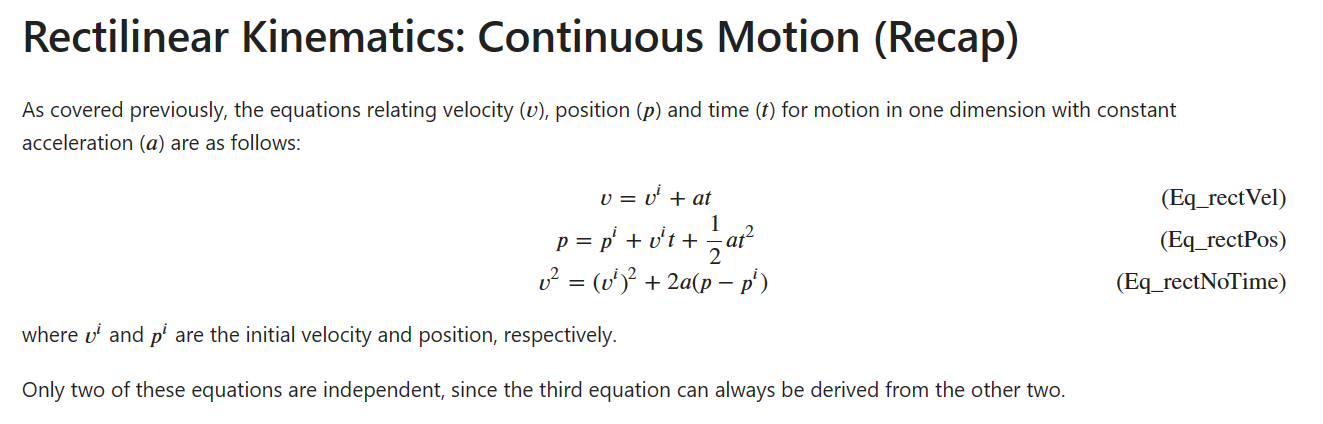
\includegraphics[width=1\textwidth]{figures/review_manual.png}
	\label{fig:review_manual}
\end{figure}

\begin{figure}[h!]
	\caption{Review Chapter Generated using Drasil}
	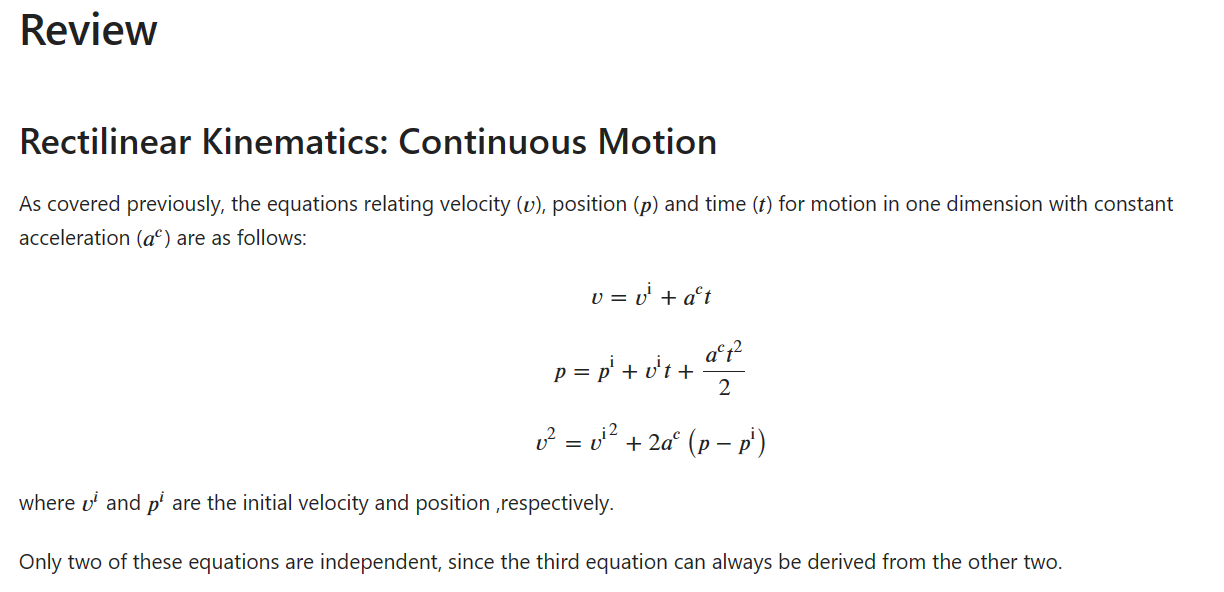
\includegraphics[width=1\textwidth]{figures/review_drasil.png}
	\label{fig:review_drasil}
\end{figure}

The remaining chapters of the generated Projectile Motion Lesson can be found 
in Appendix A, from Figure~\ref{fig:learnObj} to Figure~\ref{fig:caseProb-5}. 

\section{Knowledge Reusability}
Drasil offers the advantage of reusing knowledge, which is not trivial. We 
would like to highlight this feature with the Projectile and Projectile Motion 
Lesson. 

In Drasil, we store commonly used knowledge, such as physics concepts (e.g., 
acceleration) and mathematics ideas (e.g., Cartesian coordinates), in a package 
named \textbf{drasil-data}. Additionally, each case study has its own package 
that contains concepts specific to that study. For example, ``Projectile 
Motion" is an idea in the Projectile case study. Once these ideas and concepts 
are defined in Drasil, they can be utilized whenever needed. Since there is an 
overlap in knowledge between the Projectile SRS and Projectile Motion Lesson, 
we can reuse the information without the need to encode it again.

For example, the following equation is the position of a particle moving in a 
straight line as a function of time, given that the object experiences a 
constant acceleration:

\begin{equation}
	\label{eq:rectPos}
	p=p^i+v^it+\frac{a^ct^2}{2}
\end{equation}

On the left side of the equation, denoted as $p$ and named as 
\texttt{scalarPos}, is a physical quantity with units as a \texttt{UnitalChunk} 
defined in \textbf{drasil-data}. On the right side, we have an expression 
denoted as \texttt{scalarPos'}, declared as a \texttt{PExpr} in the Projectile 
package in \textbf{drasil-example}, as shown in Code~\ref{code:scalarPos}. 

\begin{listing}[h!]
	\caption{Source Code for scalarPos} 
	\label{code:scalarPos}
	\begin{lstlisting}[language=haskell1]		
		scalarPos :: UnitalChunk
		scalarPos  = uc CP.scalarPos lP Real metre
		
		scalarPos' :: PExpr
		scalarPos' = sy iPos `addRe` (sy QP.iSpeed `mulRe` 
		sy time `addRe` half (sy QP.constAccel `mulRe` square (sy time)))
	\end{lstlisting}
\end{listing}

The information of Equation~\ref{eq:rectPos} was already available prior to 
the development of Projectile Motion. By utilizing the definitions of both 
\texttt{scalarPos} and \texttt{scalarPos'} as a reference, we can incorporate 
this information into our own usage for the lesson plan. The implementation of 
this can be seen in Code~\ref{code:lcrectPos}. The expression is defined in a 
\texttt{LabelledContent} because we are adding a label to it, allowing us to 
cross-reference it in the document.

\begin{listing}[h!]
	\caption{Source Code for lcrectPos} 
	\label{code:lcrectPos}
	\begin{lstlisting}[language=haskell1]		
		lcrectPos :: LabelledContent
		lcrectPos = lbldExpr (sy scalarPos $= scalarPos') (makeEqnRef "rectPos")
	\end{lstlisting}
\end{listing}

Drasil offers a powerful way to store and reuse knowledge across different 
domains and aspects of the case study. By growing our knowledge database in 
this way, we believe that we can save time and effort while also ensuring 
consistency and accuracy in the use of concepts and ideas. This has the 
potential to greatly enhance the efficiency and effectiveness of engineering 
projects, and we are excited to continue exploring the possibilities of Drasil 
in the field of engineering.
\chapter{Code Block Generation} \label{chap:codeBlock}
Jupyter Notebooks are valued for their effectiveness in writing and revising 
code for data research. They allow code to be written in discrete blocks (or 
``cells"), which can be executed separately, as opposed to writing and running 
a whole program \cite{jupyterNotebookUsage}. This allows for a mix of content 
types, including equations, figures, and graphs, with code to better present 
information. 

In Chapter~\ref{chap:nbprinter}, we cover two types of metadata in Jupyter 
Notebooks: one type is necessary for forming the notebook, while the other is 
required to create cells for the contents. We explain how to generate the 
metadata and create a Markdown cell. When generating the SRS, we do not need to 
worry about generating code blocks since the SRS does not include any code. 
However, when creating lesson plans (or user manuals), we likely want to 
integrate real examples that involve code. As we are now combining text and 
code in a document, we need to address the following questions before 
generating the right type of cell: i) what type of cell should we use, Markdown 
or code? and ii) how do we know when to end a cell and start a new one? That 
is, how do we determine where to split the contents into cells?
 
To begin, we need to consider the conceptual definition of a cell in Jupyter 
Notebooks. A cell is essentially a standalone unit of information or code that 
can be executed independently. In other words, it is a unit of content within 
the notebook \cite{cellsseparation}. A cell can contain either text or code and 
can span multiple lines. Understanding the relationship between cells and their 
contents is crucial for implementing an effective splitting strategy. By 
identifying natural boundaries within the text or code and recognizing the unit 
of the contents, we can determine where to split the contents into cells.

In this chapter, we will discuss different approaches and implementations for 
splitting the contents and generating the appropriate type of cells.

\section{Unit of Contents}
To organize the contents of a lesson plan, we use two different approaches: by 
sections and by content types. We will discuss the advantages and disadvantages 
of these approaches.

\subsection{Section-level}
When considering what would be the appropriate unit of content for splitting, 
one might first think of paragraphs or sections. In the source language of 
Drasil, since a document is made up of sections (as seen in 
Code~\ref{code:drasil-lang-document}), it may appear reasonable to split these 
sections into individual cells. However, the nested structure of Drasil 
documents, where each \texttt{Section} is composed of a list of 
\texttt{Contents} and \texttt{Section}s (as demonstrated in 
Code~\ref{code:section}), does not align well with the sequential flow of a 
Jupyter Notebook. To address this issue, we flatten the structure of the Drasil 
document by making each section and subsection an independent 
\texttt{Section}. 

We have updated the definition of \texttt{Section} data type 
(Code~\ref{code:newoldsection}). In the new definition (line 9-16), the 
\texttt{Depth} attribute is used to keep track of the level of each section, 
with 0 indicating the parent section, 1 indicating the subsection, 2 indicating 
the sub-subsection, and so on. Furthermore, we have replaced the 
\texttt{SecCons} attribute, which previously represented both sections and 
contents, with a new attribute that allows each section to only have contents. 

For example, Code~\ref{code:IntroSec} defines the Introduction 
section, where 
the original nested structure (lines 1-12) comprises a list of subsections, 
while in the flattened version (lines 13-21), each subsection is self-contained 
and has its own type. Code~\ref{code:DocSection} further illustrates that each 
section is independent after the changes.

\begin{listing}[h]
	\caption{Nested and Flattened Section Comparison}
	\label{code:newoldsection}
	\begin{lstlisting}[language=haskell1]
		-- Nested Structure
		data Section = Section
							   { tle  :: Title
							   , cons :: [SecCons]
							   , _lab :: Reference
							   }
		makeLenses ''Section
		
		-- Flattened Structure
		data Section = Section 
							  { dep  :: Depth 
							  , tle  :: Title
							  , cons :: [Contents]
							  , _lab :: Reference
							  }
		makeLenses ''Section
	\end{lstlisting}
\end{listing}

\begin{listing}[h]
	\caption{Nested and Flattened Introduction Comparison}
	\label{code:IntroSec}
	\begin{lstlisting}[language=haskell1]
		-- Nested Structure
		-- | Introduction section. Contents are top level 
		-- followed by a list of subsections.
		data IntroSec = IntroProg Sentence Sentence [IntroSub]
		
		-- | Introduction subsections.
		data IntroSub where
			IPurpose :: [Sentence] -> IntroSub
			IScope   :: Sentence -> IntroSub
			IChar    :: [Sentence] -> [Sentence] -> [Sentence] -> IntroSub
			IOrgSec  :: Sentence -> CI -> Section -> Sentence -> IntroSub
	
		-- Flattened Structure
		-- | Introduction section.
		data IntroSec = IntroProg Sentence Sentence
	
		-- | Introduction subsections.
		newtype IPurpose = IPurposeProg [Sentence] 
		newtype IScope = IScopeProg Sentence 
		data IChar = ICharProg [Sentence] [Sentence] [Sentence]
		data IOrgSec = IOrgProg Sentence CI Section Sentence
	\end{lstlisting}
\end{listing}

\begin{listing}[h]
	\caption{Pseudocode for Definition of DocSection}
	\label{code:DocSection}
	\begin{lstlisting}[language=haskell1]
		-- Nested Structure
		data DocSection = TableOfContents
										| RefSec RefSec
										| IntroSec IntroSec
										| StkhldrSec StkhldrSec
										...
		
		-- Flatten Structure
		data DocSection = TableOfContents TableOfContents
										| RefSec RefSec
										| TUnits TUnits
										| TSymb TSymb
										| TAandA TAandA
										| IntroSec IntroSec
										| IPurposeSub IPurposeSub
										| IScopeSub IScopeSub
										| ICharSub ICharSub
										| IOrgSub IOrgSub
										...
		
	\end{lstlisting}
\end{listing}
 
While flattening the structure of a document can allow for it to be split into 
individual cells by sections, there are limitations to this approach. Splitting 
the contents at the section level might not always be the most effective 
approach. It's possible that certain sections might be too long to fit 
comfortably in a single cell. Moreover, when working with documents that 
combine text and code (such as lesson plans), section-level splitting may not 
be appropriate due to the different types of cells needed for text and code. 
Therefore, a better approach is needed, as presented in the next section.

\subsection{LayoutObj-level}
In Jupyter Notebook, a cell can be seen as a self-contained unit of 
information, and it can contain multiple types of content, such as text, code, 
and figures. To determine the appropriate unit of content for splitting, we 
need to consider the content itself and what makes sense in terms of its 
structure and organization.  Although a cell might not always be the most 
appropriate unit of content for splitting, it is somehow the lowest level of 
``display content" that conveys a coherent piece of information 
\cite{cellsseparation}. Therefore, splitting the content based on logical units 
of information might be a more effective approach rather than using sections as 
the sole criterion. 

In previous chapters, we discussed how Drasil handles different types of 
content through the use of the \texttt{RawContent} data type, which includes 
paragraphs, figures, equations, and other content types 
(Code~\ref{code:RawContent}). A Drasil \texttt{Section} can consist of a list 
of \texttt{RawContent}, allowing for the inclusion of different types of 
content within a single section. Additionally, as we saw in 
Chapter~\ref{chap:nbprinter}, the document is printed in a specific document 
language using \texttt{LayoutObj}, which is derived from \texttt{RawContent}. 
Because each content type is handled explicitly by \texttt{LayoutObj}, we can 
take advantage of this and split each type of content into its own cell.

To implement this approach, we first need to ensure that each layout object 
is generated independently and is not nested with other layout objects. In 
Chapter~\ref{chap:nbprinter}, we discussed how \texttt{RawContent} is 
translated to a printable \texttt{LayoutObj}. The \texttt{printLO} function in 
Code~\ref{code:LayoutObj} demonstrates how the printer renders each content 
type into a notebook format. However, the current format of \texttt{LayourObj} 
is designed for the SRS and may not be suitable for lesson plans. For instance, 
the \texttt{HDiv}\footnote{The \texttt{HDiv} is a printable layout object 
that's designed to create HTML documents. The main purpose is to wrap contents 
in the $<$div$>$ tag.} type wraps sections and creates an HTML $<$div$>$ tag, 
and even an equation block is translated into the \texttt{HDiv}, 
as seen in Code~\ref{code:EqnblocktoTex]}. Moreover, the \texttt{Definition} 
type is designed for the definition or model defined in the SRS and may not be 
required for lesson plans. To better accommodate lesson plan content types, we 
may need to create a new \texttt{LayoutObj} in the future when we have a 
better understanding of the lesson plan structure.

Currently, we are using the existing \texttt{LayoutObj} to translate our 
lesson plan contents into printable layout object. Since these contents are not 
code and should be in Markdown, we print each required content type 
independently into a Markdown cell. To accomplish this, we use the 
\texttt{markdownCell} function from Code~\ref{code:markdownCell}. This function 
generates the necessary metadata and creates the Markdown cell for each layout 
object, which is our unit of content. 

Code~\ref{code:printLO'} illustrates how each content type is rendered in 
notebook format in a Markdown cell. For layout objects that are not needed in 
lesson plans, we make them empty. We also separate equation blocks from 
\texttt{HDiv} with the equation tag to have more control over the structure.

\begin{listing}[h!]
	\caption{Source Code for printLO'}
	\label{code:printLO'}
	\begin{lstlisting}[language=haskell1, basicstyle=\small\ttfamily]
		-- printLO' is used for generating lesson plans
		printLO' :: LayoutObj -> Doc
		printLO' (HDiv ["equation"] layObs _) = markdownCell $ 
			vcat (map printLO' layObs)
		printLO' (Header n contents l) = markdownCell $ nbformat 
			(h (n + 1) <> pSpec contents) $$ refID (pSpec l)
		printLO' (Cell layObs) = vcat (map printLO' layObs)
		printLO' HDiv {} = empty
		printLO' (Paragraph contents) = markdownCell $ nbformat 
			(stripnewLine (show(pSpec contents)))
		printLO' (EqnBlock contents) = nbformat mathEqn
			where
				toMathHelper (PL g) = PL (\_ -> g Math)
				mjDelimDisp d = text "$$" <> stripnewLine (show d) <> text "$$" 
				mathEqn = mjDelimDisp $ printMath $ toMathHelper $ 
					TeX.spec contents
		printLO' (Table _ rows r _ _) = markdownCell $ 
			makeTable rows (pSpec r)
		printLO' (Definition dt ssPs l) = empty
		printLO' (List t) = markdownCell $ makeList t False
		printLO' (Figure r c f wp) = markdownCell $ makeFigure 
			(pSpec r) (pSpec c) (text f) wp
		printLO' (Bib bib) = markdownCell $ makeBib bib
		printLO' Graph{} = empty
	\end{lstlisting}
\end{listing}

As splitting contents by their types rather than sections makes more sense and 
better satisfies our needs, we can keep the document structure nested. Also, as 
the structure of our lesson plans is already linear, we can achieve the goal of 
breaking contents into smaller units by adopting only the second approach.

\section{Code Block}
We split contents with our content types for various reasons, including the 
need to differentiate between Markdown contents and code to generate the 
appropriate type of cell and to specifically deal with each type of content. 
To better manage and generate code in Jupyter Notebook with Drasil, we 
introduce a new content type called \texttt{CodeBlock}. Like other content 
types, a \texttt{CodeBlock} is defined within \texttt{RawContent}, which 
requires a \texttt{CodeExpr} as shown in Code~\ref{code:newRawContent}.

\begin{listing}[h!]
	\caption{Source Code for the New Definition of RawContent}
	\label{code:newRawContent}
	\begin{lstlisting}[language=haskell1]
		-- | Types of layout objects we deal with explicitly.
		data RawContent =
		Table [Sentence] [[Sentence]] Title Bool
		| Paragraph Sentence                       
		| EqnBlock ModelExpr                      
		| DerivBlock Sentence [RawContent]        
		| Enumeration ListType                    
		| Defini DType [(Identifier, [Contents])] 
		| Figure Lbl Filepath MaxWidthPercent     
		| Bib BibRef                              
		| Graph [(Sentence, Sentence)] (Maybe Width) (Maybe Height) Lbl
		| CodeBlock CodeExpr   
	\end{lstlisting}
\end{listing}

\texttt{CodeExpr} is a language (pre-existing in Drasil) that allows us to 
define code expressions. It shares similarities with \texttt{Expr} functions, 
constructors, and operators, but is tailored specifically for generating code. 
We utilize this data type to define and encode the expressions for our Jupyter 
Notebook code. 

The process of handling code blocks and printing the code within a code cell 
is similar to how we handle other Markdown contents, as discussed in the 
previous chapters. However, the conversion is unique to the \texttt{CodeBlock} 
type. For instance, to encode the code, we can use the \texttt{unlbldCode} 
(Code~\ref{code:unlbldCode}) function, which converts a \texttt{CodeExpr} to 
\texttt{Contents}.

\begin{listing}[h!]
	\caption{Source Code for Rendering CodeBlock to LayoutObj}
	\label{code:unlbldCode}
	\begin{lstlisting}[language=haskell1]
		-- | Unlabelled code expression
		unlbldCode :: CodeExpr -> Contents
		unlbldCode c = UlC $ ulcc $ CodeBlock c
	\end{lstlisting}
\end{listing}

After encoding the code expressions in Drasil, the printer then converts the 
code blocks into printable layout objects, as defined in 
Code~\ref{code:newLayoutObj}, using the methods in 
Code~\ref{code:codeBlocktoLayObj}. The resulting content, which is a 
\texttt{RawContent}, is translated into a printable object, a 
\texttt{LayoutObj}, before being processed by the document language printer. 

\begin{listing}[h!]
	\caption{Source Code for the New Definition of LayoutObj}
	\label{code:newLayoutObj}
	\begin{lstlisting}[language=haskell1]
		data LayoutObj = 
				Table Tags [[Spec]] Label Bool Caption                          
			| Header Depth Title Label                                       
			| Paragraph Contents                                              
			| EqnBlock Contents                                               
			| Definition DType [(String,[LayoutObj])] Label                   
			| List ListType                                                   
			| Figure Label Caption Filepath MaxWidthPercent                  
			| Graph [(Spec, Spec)] (Maybe Width) (Maybe Height) Caption Label 
			| CodeBlock Contents  
			| HDiv Tags [LayoutObj] Label                                    
			| Cell [LayoutObj] 
			| Bib BibRef     
	\end{lstlisting}
\end{listing}

\begin{listing}[h!]
	\caption{Source Code for Rendering CodeBlock to LayoutObj}
	\label{code:codeBlocktoLayObj}
	\begin{lstlisting}[language=haskell1]
		-- | Helper that translates 'LabelledContent's to a 
		-- printable representation of 'LayoutObj'.
		layLabelled sm (LblC _ (CodeBlock c)) = T.CodeBlock 
		(P.E (codeExpr c sm))
		-- | Helper that translates 'RawContent's to a 
		-- printable representation of 'LayoutObj'.
		layUnlabelled sm (CodeBlock c) = T.CodeBlock (P.E (codeExpr c sm))
	\end{lstlisting}
\end{listing}

Generating a code cell in Jupyter Notebook requires metadata, similar to 
generating a markdown cell. However, since the metadata is identical across 
code cells, the \texttt{codeCell} function generates the required metadata and 
creates a code cell for the given code, which is the `contents' in 
Code~\ref{code:codeBlocktoJSON}. This constructor eliminates the need for 
redundant metadata specification and provides a convenient way to generate code 
cells in Jupyter Notebook.

\begin{listing}[h!]
	\caption{Source Code for Generating a CodeBlock}
	\label{code:codeBlock}
	\begin{lstlisting}[language=haskell1]		
		-- | Helper for generate a Code cell
		codeCell :: Doc -> Doc
		codeCell c = codeB <> c <> codeE
		
		codeB, codeE :: Doc
		codeB = text "  {\n   \"cell_type\": \"code\",\n   
			\"execution_count\": null,\n   \"metadata\": 
			{},\n   \"outputs\": [],\n   \"source\": [" 
		codeE  = text "\n   ]\n  },"
		\end{lstlisting}
\end{listing}

Finally, the JSON printer takes the printable layout object of the code block, 
prints the code, converts it to the notebook format, and generates a code cell, 
as demonstrated in Code~\ref{code:codeBlocktoJSON}.

\begin{listing}[h!]
	\caption{Source Code for Rendering CodeBlock into JSON}
	\label{code:codeBlocktoJSON}
	\begin{lstlisting}[language=haskell1]
		-- | Helper for rendering CodeBlock into JSON
		printLO' (CodeBlock contents) = codeCell $ nbformat $ cSpec contents
	\end{lstlisting}
\end{listing}

The benefits of using Jupyter Notebook lie in its ability to allow users to 
write a portion of code and combine it with text. We have discussed various 
approaches to split the contents and generate the appropriate types of cell. 
The Projectile Motion Lesson generated by Drasil (an snapshot of the example 
chapter is shown in Figure~\ref{fig:example_drasil}), demonstrates that we are 
able to mix text and code and generate the appropriate cell types in Jupyter 
Notebook with Drasil. The source code for encoding this example can be found in 
Code~\ref{code:encodeExample}. In comparison, Figure~\ref{fig:example_manual} 
shows the same part created manually.

\begin{figure}[h!]
	\caption{Snapshot of Example Chapter Generated using Drasil}
	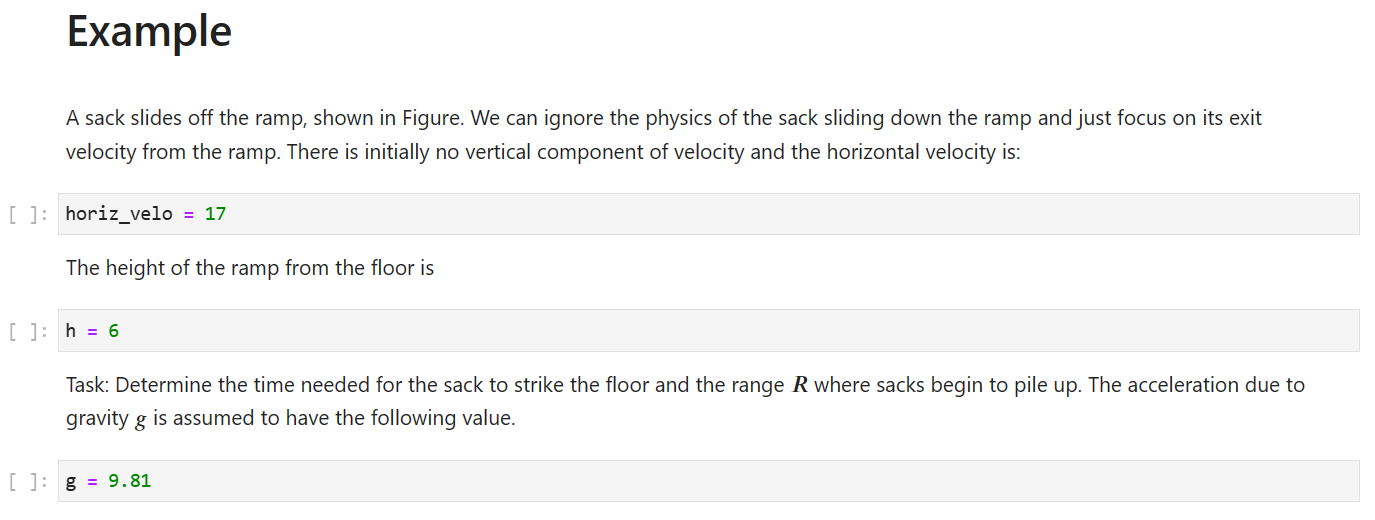
\includegraphics[width=1\textwidth]{figures/example_drasil.png}
	\label{fig:example_drasil}
\end{figure}

\begin{figure}[h!]
	\caption{Snapshot of Example Chapter Created Manually}
	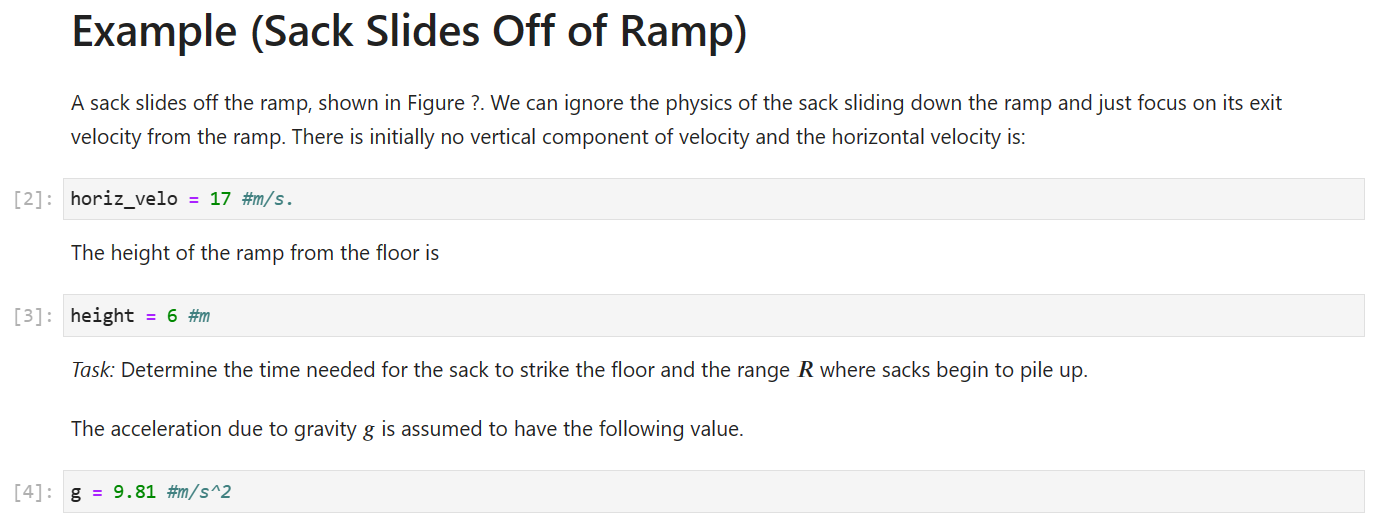
\includegraphics[width=1\textwidth]{figures/example_manual.png}
	\label{fig:example_manual}
\end{figure}

\begin{listing}[h!]
	\caption{Source Code for Encoding Example Chapter}
	\label{code:encodeExample}
	\begin{lstlisting}[language=haskell1]
	exampleContent :: [Contents]
	exampleContent = [exampleContextP1, codeC1, 
		exampleContextP2, codeC2, exampleContextP3, codeC3]
		
	exampleContextP1, exampleContextP2, exampleContextP3 :: Contents
	exampleContextP1 = foldlSP_ [S "A sack slides off the
		ramp, shown in Figure.", S "We can ignore the physics 
		of the sack sliding down the ramp and just focus on 
		its exit", phrase velocity +:+. S "from the ramp",
		S "There is initially no vertical component of", 
		phrase velocity `S.andThe` S "horizontal", 
		phrase velocity, S "is:"]
	exampleContextP2 = foldlSP_ [S "The", phrase height 
		`S.ofThe` S "ramp from the floor is"]
	exampleContextP3 = foldlSP_ [S "Task: Determine the", 
		phrase time, S "needed for the sack to strike the 
		floor and the range", P cR +:+. S "where sacks begin 
		to pile up", S "The", phrase acceleration, S "due to", 
		phrase gravity, P lG +:+. S "is assumed to have the 
		following value"]
		
	codeC1, codeC2, codeC3 :: Contents
	codeC1 = unlbldCode (sy horiz_velo $= exactDbl 17)
	codeC2 = unlbldCode (sy QP.height $= exactDbl 6)
	codeC3 = unlbldCode (sy QP.gravitationalAccel $= dbl 9.81)
	\end{lstlisting}
\end{listing}
\chapter{Conclusion} \label{chap:conclusion}
In this chapter, we will discuss the future work and summarize the achievements 
of this paper.

\section{Future Work}
Although this work has contributed to the Drasil research project and opened up 
new possibilities for future research, there is still much to be done.

\subsection{JSON Printer Improvement} \label{chap:jsonPrinterImprove}
While the current JSON printer is capable of generating Jupyter Notebook 
documents, there are several issues that need to be addressed. For example, the 
JSON printer currently relies on the TeX printer function for generating 
mathematical equations. However, this approach has some limitations, and some 
equations may not be displayed correctly in Jupyter Notebook, such as the use 
of the \textbf{symbf} command for math equations in LaTeX, which is not 
valid in Jupyter 
Notebook\footnote{\href{https://github.com/JacquesCarette/Drasil/issues/2761}{symbf
 not recognized in notebook.}}. To ensure mathematical symbols and expressions 
are 
displayed correctly, it is crucial to understand how Jupyter Notebook works 
with these elements. It may be necessary to modify the JSON printer and use 
different methods or consider using specialized libraries or tools designed for 
generating mathematical equations in Jupyter Notebook. 

\subsection{Design Lesson Plan Content Type} \label{chap:designContentType}
In Chapter~\ref{chap:codeBlock}, we discussed the potential limitations of the 
current \texttt{LayoutObj} for the structure of lesson plans. Most of the 
existing layout objects are designed for SRS data types such as 
\texttt{Definition}. To better accommodate the content types found in lesson 
plans, we could define a new set of \texttt{LayoutObj}s that are specific to 
these types of contents, such as a model that includes step-by-step 
instructions, since many lessons include these instructions. By doing so, we 
could ensure that each content type is handled explicitly by the appropriate 
\texttt{LayoutObj}, and we could create a separate cell for each type of 
content as discussed earlier. This approach would make it easier to split the 
content into logical units of information, and it would also make the resulting 
notebook more modular and easier to navigate.

\subsection{Develop the Structure of Lesson Plans} 
\label{chap:developlsnPlanStruc}
The current structure of lesson plans includes several chapters such as 
learning objectives, case problems, and examples, and each chapter is made up 
of a list of contents. However, this structure needs improvement to better fit 
the architecture of each chapter. By gaining a better understanding of our 
lesson plans and the structure of each chapter, we can incorporate the newly 
designed specific content types (as discussed in \ref{chap:designContentType}) 
into each chapter. For example, the Case Problem chapter should include the 
model of procedure analysis, which includes step-by-step instructions. Having a 
more detailed and adaptable structure of lesson plans would enable greater 
consistency and efficiency in creating and delivering content. Furthermore, it 
would make it easier to capture the key elements and knowledge of each lesson.

\subsection{Develop the Language of Code Block}
As we have discussed in earlier chapters, Drasil has the capability to generate 
source code as a part of software artifacts. To generate code content, we can 
use the available code expression, known as \texttt{CodeExpr}. However, 
generating code in a `text' document is different from generating it as a 
program. While we can generate code and code blocks in the Jupyter Notebook, 
the current language is not yet mature and requires further improvement. For 
example, to encode the code variable, we need to define it as a 
\texttt{UnitalChunk} (Code~\ref{code:horiz_velo}) before we can use it in an 
expression. However, \texttt{UnitalChunk}s are concepts with quantities that 
require unit definition, which does not align with the concept of code 
variables. We can introduce a new data type that better fits code variables or 
create smart constructors. In addition, we still need to explore how to make 
the most of our \texttt{CodeBlock}, and generate code flawlessly. These are 
interesting areas to investigate.

\begin{listing}[h!]
	\caption{Source Code for horiz\_velo}
	\label{code:horiz_velo}
	\begin{lstlisting}[language=haskell1]
		horiz_velo :: UnitalChunk
		horiz_velo = uc horizontalMotion (variable "horiz_velo") Real velU 
	\end{lstlisting}
\end{listing}

\subsection{Enable Other Programming Languages in Notebook}
Jupyter Notebook can handle code written in multiple programming languages, 
such as Python, Matlab, Julia, and R. In Chapter~\ref{chap:nbprinter}, we cover 
the metadata required to configure the notebook's environment. At present, the 
metadata enables Python code, but we aim to support additional languages in the 
future. To accomplish this, users should be able to choose their preferred 
language, and we can generate the appropriate metadata accordingly. 
Furthermore, we need to develop the syntax or structure for supporting other 
programming languages as well.

\section{Conclusion}
This paper demonstrates the potential of Jupyter Notebook as a versatile 
tool for creating and sharing scientific documents and for enhancing the 
teaching and learning efficiency in engineering education. To extend the 
capabilities of Jupyter Notebook to Drasil, we present the implementation of 
a JSON printer that is capable of generating Drasil software artifacts, 
such as the SRS, in the notebook format. We discuss the necessary functions and 
data types for working with notebook generation, as well as the process of 
encoding information in Drasil and generating and printing Jupyter Notebook 
documents using the printer.

The addition of the JSON printer expands the application of Drasil, making it 
possible to generate educational documents and develop lesson planes. We 
analyze the similarities and differences of elements in textbook chapters to 
create a universal structure that fits our lesson plans the most and provide 
insights into the design and implementation of the structure in the Drasil 
language. With the lesson plan structure in place, we demonstrate how the 
knowledge can be manipulated and reused in Drasil through the creation of a new 
case study on Projectile Motion Lesson. 

Furthermore, we highlight the benefits of using Jupyter Notebooks for data 
research and how they enable users to seamlessly combine different content 
types with code. When creating lesson plans that involve code, we need to 
address questions such as which type of cell to use and how to determine where 
to split the contents into cells. By understanding the conceptual definition of 
a cell and identifying natural boundaries within the text or code, we can 
effectively divide the contents and generate appropriate cell types. We cover 
the implementation of Markdown and code cell generation, which are essential 
components for creating a Jupyter Notebook document. 

In conclusion, this research addresses three main problems and provides a 
starting point for generating Jupyter Notebook in Drasil. With further 
refinement and development of the JSON printer and the language of lesson 
plans, generating Jupyter Notebook documents in Drasil can open up more 
possibilities.             

   \appendix
\chapter{Appendix}
This section includes the full implementation of the JSON printer, as well as 
the language for lesson plans, and additional information to provide further 
clarification on the report.

\newpage

\label{appendix_a}
\captionof{listing}{JSON Code of a Notebook Document
	\label{code:notebookmetada}}
	\begin{lstlisting}[language=json, 
	basicstyle=\linespread{1.1}\small\ttfamily] 
		{
			"cells": [
			{
				"cell_type": "markdown",
				"metadata": {},
				"source": []
			}
			],
			"metadata": {
				"kernelspec": {
					"display_name": "Python 3",
					"language": "python",
					"name": "python3"
				},
				"language_info": {
					"codemirror_mode": {
						"name": "ipython",
						"version": 3
					},
					"file_extension": ".py",
					"mimetype": "text/x-python",
					"name": "python",
					"nbconvert_exporter": "python",
					"pygments_lexer": "ipython3",
					"version": "3.9.1"
				}
			},
			"nbformat": 4,
			"nbformat_minor": 4
		}	
	\end{lstlisting}

\newpage

\captionof{listing}{Source Code for Language.Drasil.JSON.Print
\label{code:JSONPrint}}
\begin{lstlisting}[language=haskell1, 
	basicstyle=\linespread{1.1}\small\ttfamily]
	-- | Defines .json printers to generate Jupyter Notebooks
	
	-- | Generate a python notebook document (using json).
	-- build : build the SRS document in JSON format
	-- build': build the Jupyter Notbooks (lesson plans)
	genJSON :: PrintingInformation -> DocType -> L.Document -> Doc
	genJSON sm Jupyter doc = build (makeDocument sm doc)
	genJSON sm _       doc = build' (makeDocument sm doc)
		
	-- | Build the JSON Document, called by genJSON
	build :: Document -> Doc
	build (Document t a c) = 
		markdownB $$
		nbformat (text "# " <> pSpec t) $$
		nbformat (text "## " <> pSpec a) $$
		markdownE $$
		print' c $$
		markdownB' $$
		markdownE' $$
		makeMetadata $$
		text "}" 

	build' :: Document -> Doc
	build' (Document t a c) = 
		markdownB $$
		nbformat (text "# " <> pSpec t) $$
		nbformat (text "## " <> pSpec a) $$
		markdownE $$
		markdownB' $$ 
		print c $$
		markdownE' $$
		makeMetadata $$
		text "}" 

	-- | Helper for rendering a D from Latex print
	printMath :: D -> Doc
	printMath = (`runPrint` Math)
		
	-- | Helper for rendering LayoutObjects into JSON
	-- printLO is used for generating SRS
	printLO :: LayoutObj -> Doc
	printLO (Header n contents l) = nbformat empty $$ nbformat 
		(h (n + 1) <> pSpec contents) $$ refID (pSpec l)
	printLO (Cell layoutObs) = markdownCell $ vcat (map printLO layoutObs)
	printLO (HDiv _ layoutObs _) = vcat (map printLO layoutObs)
	printLO (Paragraph contents) = nbformat empty $$ nbformat 
		(stripnewLine (show(pSpec contents)))
	printLO (EqnBlock contents) = nbformat mathEqn
		where
			toMathHelper (PL g) = PL (\_ -> g Math)
			mjDelimDisp d  = text "$$" <> stripnewLine (show d) <> text "$$" 
			mathEqn = mjDelimDisp $ printMath $ toMathHelper $ TeX.spec contents
	printLO (Table _ rows r _ _) = nbformat empty $$ 
		makeTable rows (pSpec r)
	printLO (Definition dt ssPs l) = nbformat (text "<br>") $$ 
		makeDefn dt ssPs (pSpec l)
	printLO (List t) = nbformat empty $$ makeList t False
	printLO (Figure r c f wp) = makeFigure (pSpec r) (pSpec c) (text f) wp
	printLO (Bib bib) = makeBib bib
	printLO Graph{} = empty 
	printLO CodeBlock {} = empty
		
	-- printLO' is used for generating lesson plans
	printLO' :: LayoutObj -> Doc
	printLO' (HDiv ["equation"] layoutObs _) = markdownCell $ 
		vcat (map printLO' layoutObs)
	printLO' (Header n contents l) = markdownCell $ nbformat 
		(h (n + 1) <> pSpec contents) $$ refID (pSpec l)
	printLO' (Cell layoutObs) = vcat (map printLO' layoutObs)
	printLO' HDiv {} = empty
	printLO' (Paragraph contents) = markdownCell $ nbformat
		(stripnewLine (show(pSpec contents)))
	printLO' (EqnBlock contents) = nbformat mathEqn
		where
			toMathHelper (PL g) = PL (\_ -> g Math)
			mjDelimDisp d  = text "$$" <> stripnewLine (show d) <> text "$$" 
			mathEqn = mjDelimDisp $ printMath $ toMathHelper $ TeX.spec contents
	printLO' (Table _ rows r _ _) = markdownCell $ makeTable rows (pSpec r)
	printLO' Definition {} = empty
	printLO' (List t) = markdownCell $ makeList t False
	printLO' (Figure r c f wp) = markdownCell $ 
		makeFigure (pSpec r) (pSpec c) (text f) wp
	printLO' (Bib bib) = markdownCell $ makeBib bib
	printLO' Graph{} = empty 
	printLO' (CodeBlock contents) = codeCell $ codeformat $ cSpec contents
	
	-- | Called by build
	print :: [LayoutObj] -> Doc
	print = foldr (($$) . printLO) empty
	
	-- | Called by build'
	print' :: [LayoutObj] -> Doc
	print' = foldr (($$) . printLO') empty
	
	pSpec :: Spec -> Doc
	pSpec (E e) = text "$" <> pExpr e <> text "$"
	pSpec (a :+: b) = pSpec a <> pSpec b
	pSpec (S s) = either error (text . concatMap escapeChars) $ 
		L.checkValidStr s invalid
		where
			invalid = ['<', '>']
			escapeChars '&' = "\\&"
			escapeChars c = [c]
	pSpec (Sp s) = text $ unPH $ L.special s
	pSpec HARDNL = empty
	pSpec (Ref Internal r a) = reflink r $ pSpec a
	pSpec (Ref (Cite2 n) r a) = reflinkInfo r (pSpec a)(pSpec n)
	pSpec (Ref External r a) = reflinkURI r $ pSpec a
	pSpec EmptyS    = text ""
	pSpec (Quote q) = doubleQuotes $ pSpec q
	
	cSpec :: Spec -> Doc
	cSpec (E e)  = pExpr e 
	cSpec _      = empty
	
	-- | Renders expressions in JSON 
	-- (called by multiple functions)
	pExpr :: Expr -> Doc
	pExpr (Dbl d)        = text $ showEFloat Nothing d ""
	pExpr (Int i)        = text $ show i
	pExpr (Str s)        = doubleQuotes $ text s
	pExpr (Div n d)      = mkDiv "frac" (pExpr n) (pExpr d)
	pExpr (Row l)        = hcat $ map pExpr l
	pExpr (Ident s)      = text s
	pExpr (Label s)      = text s
	pExpr (Spec s)       = text $ unPH $ L.special s
	pExpr (Sub e)        = unders <> pExpr e
	pExpr (Sup e)        = hat <> pExpr e
	pExpr (Over Hat s)   = pExpr s <> text "&#770;"
	pExpr (MO o)         = text $ pOps o
	pExpr (Fenced l r e) = text (fence Open l) <> pExpr e <> 
		text (fence Close r)
	pExpr (Font Bold e)  = pExpr e
	pExpr e              = printMath $ toMath $ TeX.pExpr e
	
	-- | Renders operations in Markdown format
	pOps :: Ops -> String
	pOps IsIn     = "&thinsp;&isin;&thinsp;"
	pOps Integer  = "&#8484;"
	pOps Rational = "&#8474;"
	pOps Real     = "&#8477;"
	pOps Natural  = "&#8469;"
	pOps Boolean  = "&#120121;"
	pOps Comma    = ","
	pOps Prime    = "&prime;"
	pOps Log      = "log"
	pOps Ln       = "ln"
	pOps Sin      = "sin"
	pOps Cos      = "cos"
	pOps Tan      = "tan"
	pOps Sec      = "sec"
	pOps Csc      = "csc"
	pOps Cot      = "cot"
	pOps Arcsin   = "arcsin"
	pOps Arccos   = "arccos"
	pOps Arctan   = "arctan"
	pOps Not      = "&not;"
	pOps Dim      = "dim"
	pOps Exp      = "e"
	pOps Neg      = "-"
	pOps Cross    = "&#10799;"
	pOps VAdd     = " + "
	pOps VSub     = " - "
	pOps Dot      = "&sdot;"
	pOps Scale    = ""
	pOps Eq       = " = "
	pOps NEq      = "&ne;"
	pOps Lt       = "&thinsp;&lt;&thinsp;" 
	pOps Gt       = "&thinsp;&gt;&thinsp;"
	pOps LEq      = "&thinsp;&le;&thinsp;"
	pOps GEq      = "&thinsp;&ge;&thinsp;"
	pOps Impl     = " &rArr; "
	pOps Iff      = " &hArr; "
	pOps Subt     = " - "
	pOps And      = " &and; "
	pOps Or       = " &or; "
	pOps Add      = " + "
	pOps Mul      = ""
	pOps Summ     = "&sum"
	pOps Inte     = "&int;"
	pOps Prod     = "&prod;"
	pOps Point    = "."
	pOps Perc     = "%"
	pOps LArrow   = " &larr; "
	pOps RArrow   = " &rarr; "
	pOps ForAll   = " ForAll "
	pOps Partial  = "&part;"
	
	-- | Renders Markdown table, called by 'printLO'
	makeTable :: [[Spec]] -> Doc -> Doc
	makeTable [] _      = error "No table to print"
	makeTable (l:lls) r = refID r $$ nbformat empty $$ 
		(makeHeaderCols l $$ makeRows lls) $$ nbformat empty
	
	-- | Helper for creating table rows
	makeRows :: [[Spec]] -> Doc
	makeRows = foldr (($$) . makeColumns) empty
	
	-- | makeHeaderCols: Helper for creating table header row 
	-- (each of the column header cells)
	-- | makeColumns: Helper for creating table columns
	makeHeaderCols, makeColumns :: [Spec] -> Doc
	makeHeaderCols l = nbformat (text header) $$ 
		nbformat (text $ genMDtable ++ "|")
		where 
			header = show(text "|" <> hcat(punctuate (text "|") 
				(map pSpec l)) <> text "|")        
			c = count '|' header
			genMDtable = concat (replicate (c-1) "|:--- ")
	
	makeColumns ls = nbformat (text "|" <> hcat(punctuate 
		(text "|") (map pSpec ls)) <> text "|")
	
	count :: Char -> String -> Int
	count _ [] = 0
	count c (x:xs) 
		| c == x = 1 + count c xs
		| otherwise = count c xs
	
	-- | Renders definition tables (Data, General, Theory, etc.)
	makeDefn :: L.DType -> [(String,[LayoutObj])] -> Doc -> Doc
	makeDefn _ [] _  = error "L.Empty definition"
	makeDefn dt ps l = refID l $$ table [dtag dt] (tr (nbformat 
		(th (text "Refname")) $$ td	(nbformat(bold l))) $$ makeDRows ps)
		where dtag L.General  = "gdefn"
			    dtag L.Instance = "idefn"
			    dtag L.Theory   = "tdefn"
			    dtag L.Data     = "ddefn"
	
	-- | Helper for making the definition table rows
	makeDRows :: [(String,[LayoutObj])] -> Doc
	makeDRows [] = error "No fields to create defn table"
	makeDRows [(f,d)] = tr (nbformat (th (text f)) $$ td 
		(vcat $ map printLO d))
	makeDRows ((f,d):ps) = tr (nbformat (th (text f)) $$ td 
		(vcat $ map printLO d)) $$ makeDRows ps
	
	-- | Renders lists
	makeList :: ListType -> Bool -> Doc
	makeList (Simple items) _ = vcat $ map (\(b,e,l) -> mlref l 
		$ nbformat (pSpec b <> text ": " <> sItem e) $$ nbformat empty) items
	makeList (Desc items) bl = vcat $ map (\(b,e,l) -> pa $
		mlref l $ ba $ pSpec b <> text ": " <> pItem e bl) items
	makeList (Ordered items) bl = vcat $ map (\(i,l) -> mlref l 
		$ pItem i bl) items
	makeList (Unordered items) bl = vcat $ map (\(i,l) -> 
		mlref l $ pItem i bl) items
	makeList (Definitions items) _ = vcat $ map (\(b,e,l) -> nbformat $ li $ 
	mlref l $ pSpec b <> text " is the" <+> sItem e) items
	
	-- | Helper for setting up references
	mlref :: Maybe Label -> Doc -> Doc
	mlref = maybe id $ refwrap . pSpec
	
	-- | Helper for rendering list items
	pItem :: ItemType ->  Bool -> Doc
	pItem (Flat s) b = nbformat $ (if b then text " - " else 
		text "- ") <> pSpec s
	pItem (Nested s l) _ = vcat [nbformat $ text "- " <> 
		pSpec s, makeList l True]
		
	sItem :: ItemType -> Doc
	sItem (Flat s)     = pSpec s
	sItem (Nested s l) = vcat [pSpec s, makeList l False]
	
	-- | Renders figures in HTML
	makeFigure :: Doc -> Doc -> Doc -> L.MaxWidthPercent -> Doc
	makeFigure r c f wp = refID r $$ image f c wp
	
	-- | Renders assumptions, requirements, likely changes
	makeRefList :: Doc -> Doc -> Doc -> Doc
	makeRefList a l i = refID l $$ nbformat(i <> text ": " <> a)
	
	makeBib :: BibRef -> Doc
	makeBib = vcat .
		zipWith (curry (\(x,(y,z)) -> makeRefList z y x))
		[text $ sqbrac $ show x | x <- [1..] :: [Int]] . map renderCite
\end{lstlisting}

\newpage

\captionof{listing}{Source Code for Language.Drasil.JSON.Helpers
	\label{code:JSONHelpers}}
\begin{lstlisting}[language=haskell1, 
	basicstyle=\linespread{1.1}\small\ttfamily]
	-- | Defines helper functions for creating Jupyter Notebooks
		
	data Variation = Class | Id
	
	tr, td, figure, li, pa, ba :: Doc -> Doc
	-- | Table row tag wrapper
	tr     = wrap "tr" []
	-- | Table cell tag wrapper
	td     = wrap "td" []
	-- | Figure tag wrapper
	figure = wrap "figure" []
	-- | List tag wrapper
	li     = wrap' "li" []
	-- | Paragraph in list tag wrapper
	pa     = wrap "p" []
	-- | Bring attention to element wrapper.
	ba     = wrap "b" []
	
	ol, ul, table :: [String] -> Doc -> Doc
	-- | Ordered list tag wrapper
	ol     = wrap "ol"
	-- | Unordered list tag wrapper
	ul     = wrap "ul"
	-- | Table tag wrapper
	table  = wrap "table"
	
	nbformat :: Doc -> Doc
	nbformat s = text ("    " ++ J.encode (show s ++ "\n") ++ ",")
	
	codeformat :: Doc -> Doc
	codeformat s = text ("    " ++ J.encode (show s))
	
	wrap :: String -> [String] -> Doc -> Doc
	wrap a = wrapGen' vcat Class a empty
	
	wrap' :: String -> [String] -> Doc -> Doc
	wrap' a = wrapGen' hcat Class a empty
	
	wrapGen' :: ([Doc] -> Doc) -> Variation -> String -> Doc -> 
		[String] -> Doc -> Doc
	wrapGen' sepf _ s _ [] = \x -> 
		let tb c = text $ "<" ++ c ++ ">"
		in if s == "li" then sepf [tb s, x, tb $ '/':s] 
			else sepf [nbformat(tb s), x, nbformat(tb $ '/':s)]
	wrapGen' sepf Class s _ ts = \x ->
		let tb c = text $ "<" ++ c ++ " class=\\\"" ++ foldr1 (++) 
			(intersperse " " ts) ++ "\\\">"
		in let te c = text $ "</" ++ c ++ ">"
		in sepf [nbformat(tb s), x, nbformat(te s)]
	wrapGen' sepf Id s ti _ = \x ->
		let tb c = text ("<" ++ c ++ " id=\\\"") <> ti <> text "\\\">"
				te c = text $ "</" ++ c ++ ">"
		in  sepf [nbformat(tb s), x, nbformat(te s)] 
	
	refwrap :: Doc -> Doc -> Doc
	refwrap = flip (wrapGen' vcat Id "div") [""]
	
	refID :: Doc -> Doc 
	refID i = nbformat $ text "<a id=\"" <> i <> text "\"></a>"
	
	-- | Helper for setting up links to references
	reflink :: String -> Doc -> Doc
	reflink ref txt = text "[" <> txt <> text ("](#" ++ ref ++ ")")
	
	-- | Helper for setting up links to external URIs
	reflinkURI :: String -> Doc -> Doc
	reflinkURI ref txt = text ("<a href=\\\"" ++ ref ++ "\\\">") 
		<> txt <> text "</a>"
	
	-- | Helper for setting up figures
	image :: Doc -> Doc -> MaxWidthPercent -> Doc
	image f c 100 = 
		figure $ vcat [
		nbformat $ img [("src", f), ("alt", c)]]
	image f c wp =
		figure $ vcat [
		nbformat $ img [("src", f), ("alt", c), ("width", 
			text $ show wp ++ "%")]]
	
	h :: Int -> Doc
	h n | n < 1 = error "Illegal header (too small)"
			| n > 4 = error "Illegal header (too large)"          
			| otherwise = text (hash n)
				where hash 1 = "# "
							hash 2 = "## "
							hash 3 = "### "
							hash 4 = "#### "
							hash _ = "Illegal header"
	
	-- | Curly braces.
	br :: Doc -> Doc
	br x = text "{" <> x <> text"}"
	
	mkDiv :: String -> Doc -> Doc -> Doc
	mkDiv s a0 a1 = (H.bslash <> text s) <> br a0 <> br a1
	
	stripnewLine :: String -> Doc
	stripnewLine s = hcat (map text (splitOn "\n" s))
	
	-- | Helper for building Markdown cells
	markdownB, markdownB', markdownE, markdownE' :: Doc
	markdownB  = text "{\n \"cells\": [\n  {\n   \"cell_type\": 
		\"markdown\",\n   \"metadata\": {},\n   \"source\": [\n" 
	markdownB' = text "  {\n   \"cell_type\": \"markdown\",\n   
		\"metadata\": {},\n   \"source\": [\n" 
	markdownE  = text "    \"\\n\"\n   ]\n  },"
	markdownE' = text "    \"\\n\"\n   ]\n  }\n ],"
		
	-- | Helper for building code cells
	codeB, codeE :: Doc
	codeB = text "  {\n   \"cell_type\": \"code\",\n   
		\"execution_count\": null,\n   \"metadata\": {},\n   
		\"outputs\": [],\n   \"source\": [" 
	codeE  = text "\n   ]\n  },"
		
	-- | Helper for generate a Markdown cell
	markdownCell :: Doc -> Doc
	markdownCell c = markdownB' <> c <> markdownE
		
	-- | Helper for generate a code cell
	codeCell :: Doc -> Doc
	codeCell c = codeB <> c <> codeE
		
	-- | Generate the metadata necessary for a notebook document
	makeMetadata :: Doc  
	makeMetadata = vcat [
		text " \"metadata\": {", 
		vcat[
			text "  \"kernelspec\": {", 
			text "   \"display_name\": \"Python 3\",", 
			text "   \"language\": \"python\",",
			text "   \"name\": \"python3\"", 
			text "  },"],
		vcat[
			text "  \"language_info\": {", 
			text "   \"codemirror_mode\": {", 
			text "    \"name\": \"ipython\",",
			text "    \"version\": 3",
			text "   },"],
		text "   \"file_extension\": \".py\",", 
		text "   \"mimetype\": \"text/x-python\",",
		text "   \"name\": \"python\",",
		text "   \"nbconvert_exporter\": \"python\",",
		text "   \"pygments_lexer\": \"ipython3\",",
		text "   \"version\": \"3.9.1\"",
		text "  }",
		text " },",
		text " \"nbformat\": 4,", 
		text " \"nbformat_minor\": 4" 
	]
\end{lstlisting}

\newpage

\captionof{listing}{Source Code for DocLang.Notebook
	\label{code:docLang_notebook}}
\begin{lstlisting}[language=haskell1, 
	basicstyle=\linespread{1.1}\small\ttfamily]	
	-- * Section Constructors	
	-- | Section constructors for the Lesson Plans
	intro, learnObj, review, caseProb, summary, appendix, 
		reference, example :: [Contents] -> [Section] -> Section
	intro     cs ss = section (titleize  Docum.introduction) 
		cs ss introLabel
	learnObj  cs ss = section (titleize' Docum.learnObj)    
		cs ss learnObjLabel
	review    cs ss = section (titleize  Docum.review)      
		cs ss reviewLabel
	caseProb  cs ss = section (titleize  Docum.caseProb)     
		cs ss caseProbLabel
	example   cs ss = section (titleize  Docum.example)      
		cs ss exampleLabel
	summary   cs ss = section (titleize  Docum.summary)      
		cs ss summaryLabel
	appendix  cs ss = section (titleize  Docum.appendix)     
		cs ss appendixLabel
	reference cs ss = section (titleize' Docum.reference)   
		cs ss referenceLabel
	
	--Labels--
	sectionReferences :: [Reference]
	sectionReferences = [introLabel, learnObjLabel, 
		docPurposeLabel, referenceLabel, reviewLabel, 
		appendixLabel, summaryLabel, exampleLabel]
	
	-- * Section References
	
	-- | Individual section reference labels. 
	-- Used in creating example sections for the notebook.
	introLabel, learnObjLabel, docPurposeLabel, referenceLabel, 
		reviewLabel, caseProbLabel, appendixLabel, summaryLabel, 
		exampleLabel :: Reference
	introLabel      = makeSecRef "Intro"            
		$ titleize  Docum.introduction
	learnObjLabel   = makeSecRef "LearnObj"         
		$ titleize' Docum.learnObj
	docPurposeLabel = makeSecRef "DocPurpose"       
		$ titleize  Docum.prpsOfDoc
	referenceLabel  = makeSecRef "References"       
		$ titleize'	Docum.reference
	reviewLabel     = makeSecRef "Review"           
		$ titleize  Docum.review
	caseProbLabel   = makeSecRef "CaseProb"         
		$ titleize  Docum.caseProb
	appendixLabel  = makeSecRef "Appendix"         
		$ titleize  Docum.appendix
	summaryLabel   = makeSecRef "Summary"          
		$ titleize  Docum.summary
	exampleLabel   = makeSecRef "Example"         
		$ titleize  Docum.example
\end{lstlisting}

\newpage

\captionof{listing}{Source Code for DocumentLanguage.Notebook.Core
	\label{code:notebook_Core}}
\begin{lstlisting}[language=haskell1, 
	basicstyle=\linespread{1.1}\small\ttfamily]
	module Drasil.DocumentLanguage.Notebook.Core where
	
	-- * Lesson Chapter Types
	
	type LsnDesc = [LsnChapter]
	
	data LsnChapter = Intro Intro
	| LearnObj LearnObj
	| Review Review
	| CaseProb CaseProb
	| Example Example
	| Smmry Smmry
	| BibSec
	| Apndx Apndx
	
	-- ** Introduction
	newtype Intro = IntrodProg [Contents]
	
	-- ** Learning Objectives
	newtype LearnObj = LrnObjProg [Contents]
	
	-- ** Review Chapter
	newtype Review = ReviewProg [Contents]
	
	-- ** A Case Problem
	newtype CaseProb = CaseProbProg [Contents]
	
	-- ** Examples of the lesson
	newtype Example = ExampleProg [Contents]
	
	-- ** Summary
	newtype Smmry = SmmryProg [Contents]
	
	-- ** Appendix
	newtype Apndx = ApndxProg [Contents]
	
	-- * Multiplate Definition and Type	
	data DLPlate f = DLPlate {
		lsnChap :: LsnChapter -> f LsnChapter,
		intro :: Intro -> f Intro,
		learnObj :: LearnObj -> f LearnObj,
		review :: Review -> f Review,
		caseProb :: CaseProb -> f CaseProb,
		example :: Example -> f Example,
		smmry :: Smmry -> f Smmry,
		apndx :: Apndx -> f Apndx
	}
	
	instance Multiplate DLPlate where
		multiplate p = DLPlate lc introd lrnObj rvw csProb exmp smry aps where
		lc (Intro x) = Intro <$> intro p x
		lc (LearnObj x) = LearnObj <$> learnObj p x
		lc (Review x) = Review <$> review p x
		lc (CaseProb x) = CaseProb <$> caseProb p x
		lc (Example x) = Example <$> example p x
		lc (Smmry x) = Smmry <$> smmry p x
		lc (Apndx x) = Apndx <$> apndx p x
		lc BibSec = pure BibSec
	
		introd (IntrodProg con) = pure $ IntrodProg con 
		lrnObj (LrnObjProg con) = pure $ LrnObjProg con 
		rvw (ReviewProg con) = pure $ ReviewProg con
		csProb (CaseProbProg con) = pure $ CaseProbProg con 
		exmp (ExampleProg con) = pure $ ExampleProg con
		smry (SmmryProg con) = pure $ SmmryProg con 
		aps (ApndxProg con) = pure $ ApndxProg con
		mkPlate b = DLPlate (b lsnChap) (b intro) (b learnObj) 
			(b review) (b caseProb) (b example) (b smmry) (b apndx)
\end{lstlisting}

\newpage

\captionof{listing}{Source Code for DocumentLanguage.Notebook.DocumentLanguage
	\label{code:notebook_DocumentLanguage}}
\begin{lstlisting}[language=haskell1, 
	basicstyle=\linespread{1.1}\small\ttfamily]
	-- | Creates a notebook from a lesson description and system information.
	mkNb :: LsnDecl -> (IdeaDict -> IdeaDict -> Sentence) -> 
		SystemInformation -> Document
	mkNb dd comb si@SI {_sys = s, _kind = k, _authors = a} =
		Notebook (nw k `comb` nw s) (foldlList Comma List $ 
			map (S . name) a) $
		mkSections si l where
			l = mkLsnDesc si dd
	
	-- | Helper for creating the notebook sections.
	mkSections :: SystemInformation -> LsnDesc -> [Section]
	mkSections si = map doit  
		where
			doit :: LsnChapter -> Section
			doit (Intro i)     = mkIntro i
			doit (LearnObj l)  = mkLearnObj l
			doit (Review r)    = mkReview r
			doit (CaseProb cp) = mkCaseProb cp
			doit (Example e)   = mkExample e
			doit (Smmry s)     = mkSmmry s
			doit BibSec        = mkBib (citeDB si)
			doit (Apndx a)     = mkAppndx a
	
	-- | Helper for making the 'Introduction' section.
	mkIntro :: Intro -> Section
	mkIntro (IntrodProg i) = Lsn.intro i []
	
	-- | Helper for making the 'Learning Objectives' section.
	mkLearnObj :: LearnObj -> Section
	mkLearnObj (LrnObjProg cs) = Lsn.learnObj cs []
	
	-- | Helper for making the 'Review' section.
	mkReview :: Review -> Section
	mkReview (ReviewProg r) = Lsn.review r [] 
	
	-- | Helper for making the 'Case Problem' section.
	mkCaseProb :: CaseProb -> Section
	mkCaseProb (CaseProbProg cp) = Lsn.caseProb cp [] 
	
	-- | Helper for making the 'Example' section.
	mkExample:: Example -> Section
	mkExample (ExampleProg cs) = Lsn.example cs []
	
	-- | Helper for making the 'Summary' section.
	mkSmmry :: Smmry -> Section
	mkSmmry (SmmryProg cs) = Lsn.summary cs []
	
	-- | Helper for making the 'Bibliography' section.
	mkBib :: BibRef -> Section
	mkBib bib = Lsn.reference [UlC $ ulcc (Bib bib)] []
	
	-- | Helper for making the 'Appendix' section.
	mkAppndx :: Apndx -> Section
	mkAppndx (ApndxProg cs) = Lsn.appendix cs []
\end{lstlisting}

\newpage

\captionof{listing}{Source Code for DocumentLanguage.Notebook.LsnDecl
	\label{code:notebook_LsnDecl}}
\begin{lstlisting}[language=haskell1, 
	basicstyle=\linespread{1.1}\small\ttfamily]	
	-- | A Lesson Plan notebook declaration is made up of all 
	-- necessary chapters ('LsnChapter's).
	type LsnDecl  = [LsnChapter]
	
	-- | Contains all the different chapters needed for a 
	-- notebook lesson plan ('LsnDecl').
	data LsnChapter = Intro NB.Intro
									| LearnObj NB.LearnObj
									| Review NB.Review
									| CaseProb NB.CaseProb
									| Example NB.Example
									| Smmry NB.Smmry
									| BibSec
									| Apndx NB.Apndx
	
	-- * Functions
	
	-- | Creates the lesson description (translates 'LsnDecl' 
	-- into a more usable form for generating documents).
	mkLsnDesc :: SystemInformation -> LsnDecl -> NB.LsnDesc
	mkLsnDesc _ = map sec where
		sec :: LsnChapter -> NB.LsnChapter
		sec (Intro i)    = NB.Intro i
		sec (LearnObj l) = NB.LearnObj l
		sec (Review r)   = NB.Review r  
		sec (CaseProb c) = NB.CaseProb c
		sec (Example e)  = NB.Example e  
		sec (Smmry s)    = NB.Smmry s
		sec BibSec       = NB.BibSec
		sec (Apndx a)    = NB.Apndx a
\end{lstlisting}

\begin{figure}
	\caption{Learning Objectives Generated using Drasil}
	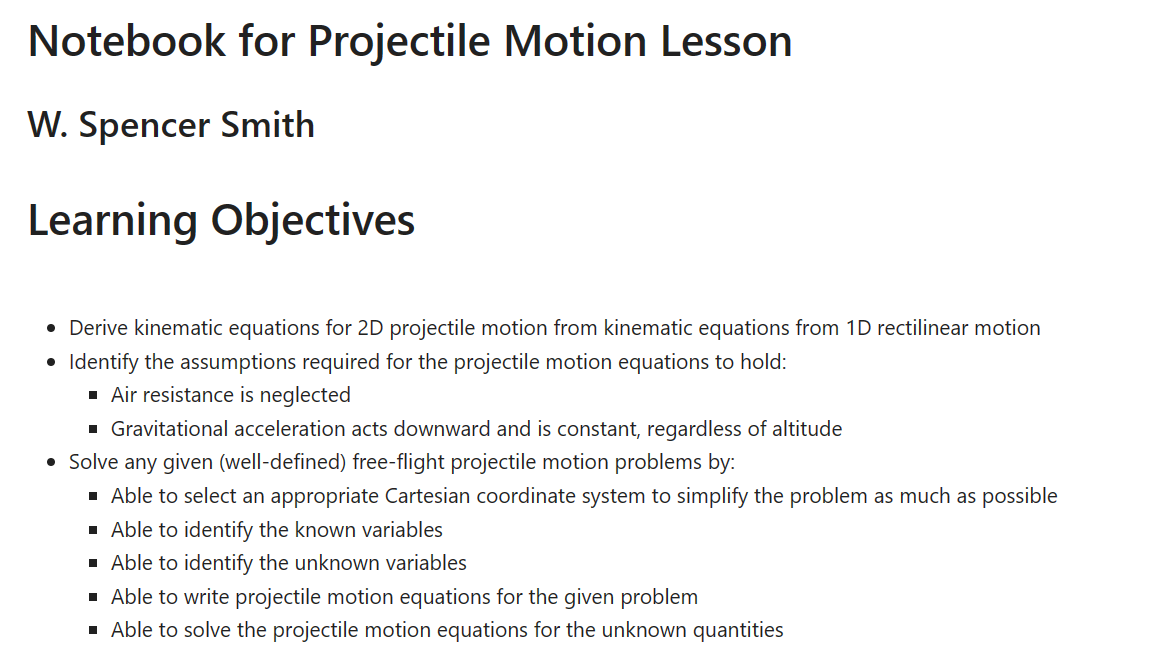
\includegraphics[width=1\textwidth]{figures/learnObj.png}
	\label{fig:learnObj}
\end{figure}

\begin{figure}[h!]
	\caption{Case Problem Generated using Drasil}
	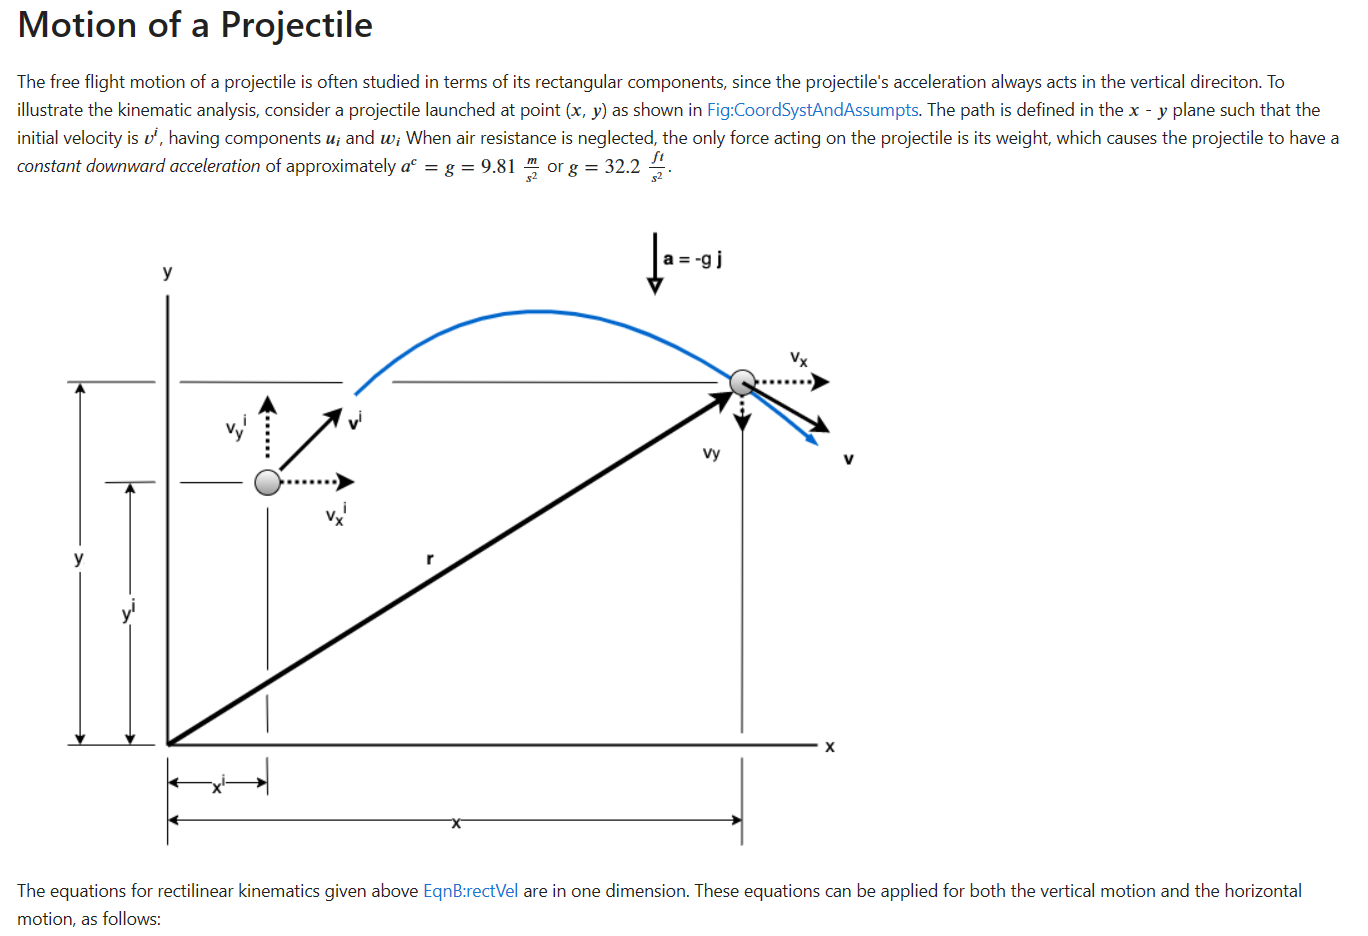
\includegraphics[width=1\textwidth]{figures/caseProb-1.png}
	\label{fig:caseProb-1}
\end{figure}

\begin{figure}[h!]
	\caption{Case Problem Generated using Drasil Cont.}
	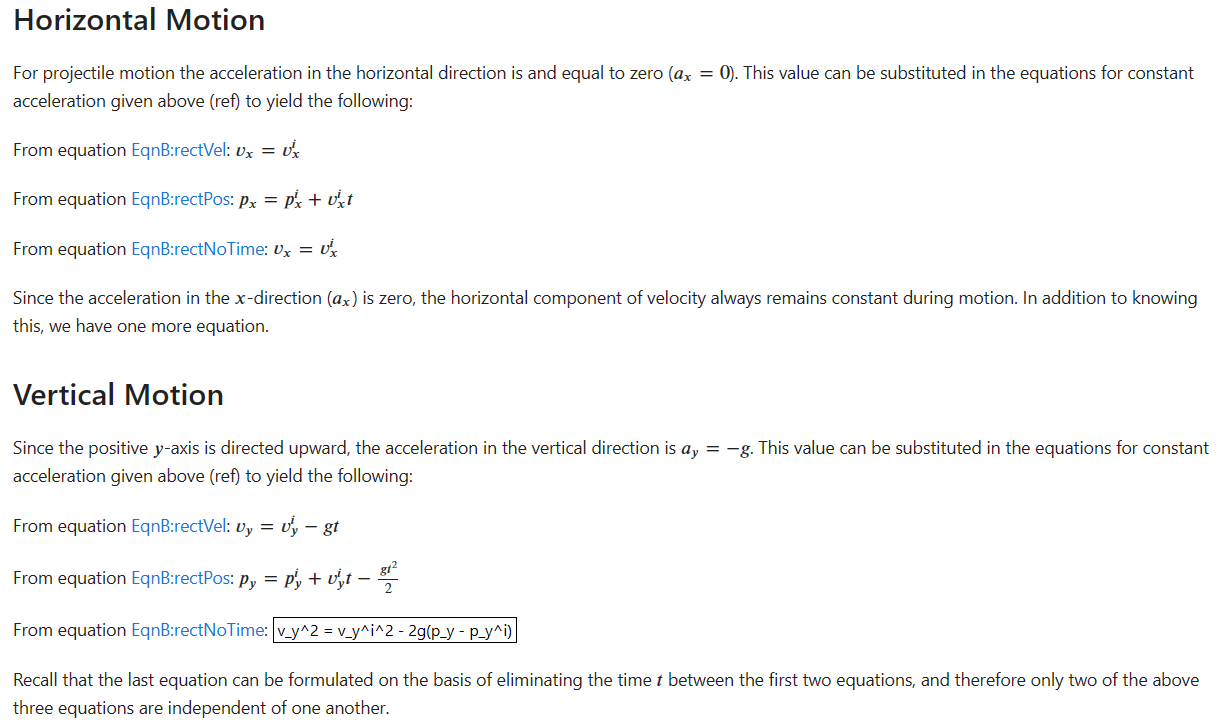
\includegraphics[width=1\textwidth]{figures/caseProb-2.png}
	\label{fig:caseProb-2}
\end{figure}

\begin{figure}[h!]
	\caption{Case Problem Generated using Drasil Cont.}
	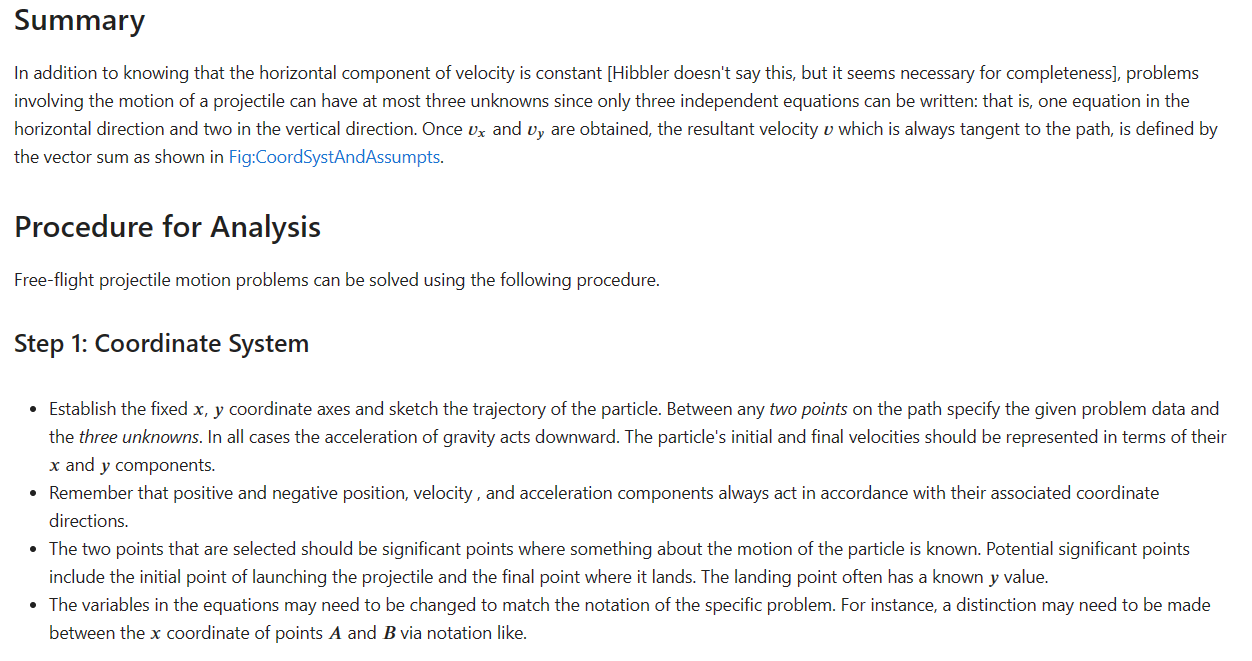
\includegraphics[width=1\textwidth]{figures/caseProb-3.png}
	\label{fig:caseProb-3}
\end{figure}

\begin{figure}[h!]
	\caption{Case Problem Generated using Drasil Cont.}
	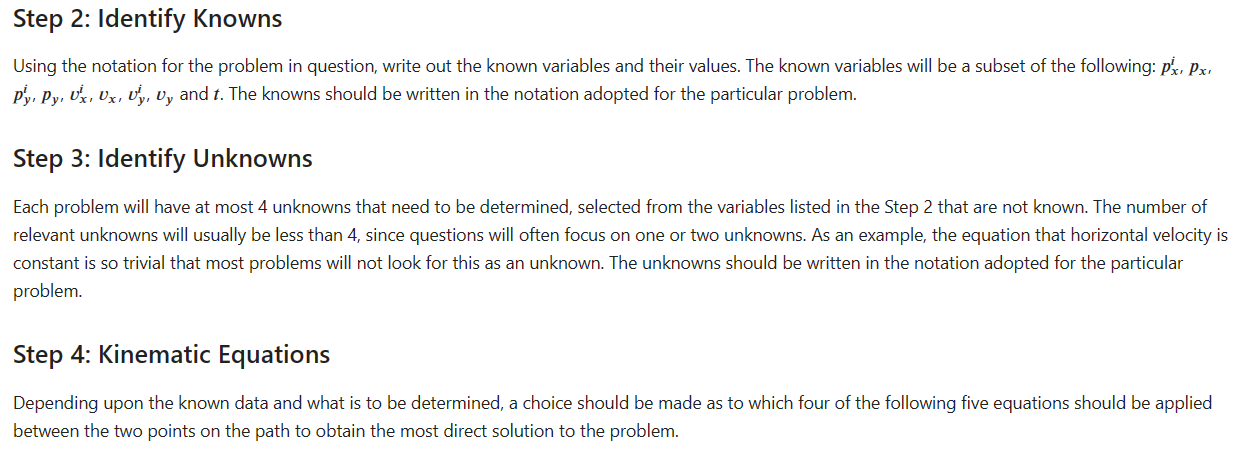
\includegraphics[width=1\textwidth]{figures/caseProb-4.png}
	\label{fig:caseProb-4}
\end{figure}

\begin{figure}[h!]
	\caption{Case Problem Generated using Drasil Cont.}
	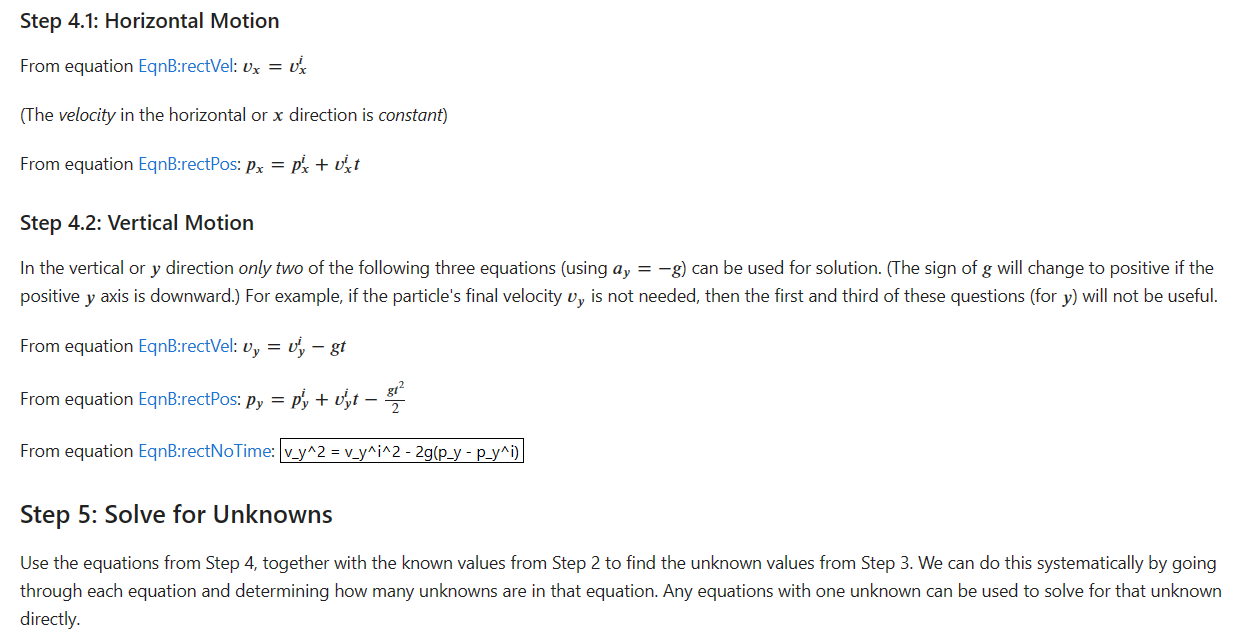
\includegraphics[width=1\textwidth]{figures/caseProb-5.png}
	\label{fig:caseProb-5}
\end{figure}



       \setcounter{figure}{0}
       \setcounter{equation}{0}
       \setcounter{table}{0}

% The bibliography is set up to allow for multiple bib files
\printbibliography

\label{NumDocumentPages}

\end{document}
% ********************************
